\RequirePackage[l2tabu,orthodox]{nag}
\documentclass[12pt,oneside,article,draft]{memoir}
% !TEX root = ./CCC_Note.tex

\usepackage{amsmath}
\usepackage{amsthm}
\usepackage{amsfonts}
\usepackage{amssymb}
\usepackage{mathtools}
%\usepackage{datetime}
\usepackage[usenames,dvipsnames]{xcolor}
\usepackage[bookmarks=true,colorlinks=true, linkcolor=MidnightBlue, citecolor=cyan]{hyperref}
\usepackage[T1]{fontenc}
\usepackage[sc]{mathpazo}
\linespread{1.05}
\usepackage{mathrsfs}
\usepackage{euscript}
%\usepackage{MnSymbol}
\usepackage{paralist}
\usepackage{todonotes}
\usepackage{makecell}
\usepackage{booktabs}
\usepackage{tikz}
\usetikzlibrary{cd}
\usepackage{tensor}

\usetikzlibrary{decorations.markings,arrows.meta,calc,fit,quotes}
\hypersetup{final}

\DeclareMathOperator{\id}{id}
\DeclareMathOperator{\dom}{dom}
\DeclareMathOperator{\cod}{cod}
\DeclareMathOperator{\dvert}{Vert}
\DeclareMathOperator{\Lax}{Lax}
\DeclareMathOperator{\Hom}{Hom}
\DeclareMathOperator{\Ob}{Ob}
\DeclareMathOperator{\Tr}{Tr}


\theoremstyle{plain}
\newtheorem{theorem}{Theorem}[section]
\newtheorem*{theorem*}{Theorem}
\newtheorem{proposition}[theorem]{Proposition}
\newtheorem{corollary}[theorem]{Corollary}
\newtheorem{lemma}[theorem]{Lemma}
\newtheorem*{lemma*}{Lemma}

\theoremstyle{definition}
\newtheorem{definition}[theorem]{Definition}
\newtheorem{exercise}{Exercise}[section]

\theoremstyle{remark}
\newtheorem{example}[theorem]{Example}
\newtheorem{remark}[theorem]{Remark}

\newcommand{\prodb}{\mathbin{\Pi}}
\newcommand{\iso}{\cong}

\newcommand{\cat}[1]{\mathscr{#1}}
\newcommand{\Cat}[1]{\mathbf{#1}}
\newcommand{\fun}[1]{#1}
\newcommand{\Fun}[1]{\mathsf{#1}}
%\newcommand{\hom}{\mathrm{hom}}
\newcommand{\twocat}[1]{\mathcal{#1}}
\newcommand{\dblcat}[1]{\mathbb{#1}}
\newcommand{\Mon}{\Cat{Mon}}
\newcommand{\Prof}{\Cat{Prof}}
\newcommand{\MProf}{\Cat{MProf}}
\newcommand{\MonCat}{\Cat{MonCat}}
\newcommand{\SymMonCat}{\Cat{SymMonCat}}
\newcommand{\CompCat}{\Cat{CompCat}}
\newcommand{\TrCat}{\Cat{TrCat}}
\newcommand{\Set}{\Cat{Set}}
\newcommand{\Int}{\Fun{Int}}

\newcommand{\op}[1]{{#1}^{\text{op}}}
\newcommand{\vop}[1]{{#1}^{\text{vop}}}
\newcommand{\hop}[1]{{#1}^{\text{hop}}}

\newcommand{\Alg}{\mathrm{Alg}}
\newcommand{\Coalg}{\mathrm{Coalg}}
\newcommand{\RAlg}[1][]{\mathbb{R}_{#1}\text{-}\Alg}
\newcommand{\LCoalg}[1][]{\mathbb{L}_{#1}\text{-}\Coalg}
\newcommand{\LCoalgA}{\mathbb{L}_1\text{-}\Coalg}
\newcommand{\LCoalgB}{\mathbb{L}_2\text{-}\Coalg}

\newcommand{\twocell}[3][]{\arrow[draw=none,to path={(dom#2.center)--(cod#2.center)\tikztonodes}]{}[anchor=center,#1]{\Downarrow #3}}
\newcommand{\twocellalt}[3][]{\arrow[draw=none,to path={(dom#2.center)--(cod#2.center)\tikztonodes}]{}[anchor=center,#1]{#3}}
\newcommand{\twocellA}[2][]{\twocell[#1]{A}{#2}}
\newcommand{\twocellB}[2][]{\twocell[#1]{B}{#2}}
\newcommand{\twocellC}[2][]{\twocell[#1]{C}{#2}}
\newcommand{\twocellD}[2][]{\twocell[#1]{D}{#2}}
\newcommand{\twocellE}[2][]{\twocell[#1]{E}{#2}}
\newcommand{\twocellF}[2][]{\twocell[#1]{F}{#2}}



\tikzcdset{
	arrow style=tikz,
	diagrams={>={Classical TikZ Rightarrow[angle=63:4pt, line width=.6pt]}},
	arrows={semithick}
}

\tikzset{tick/.style={postaction={decorate,decoration={markings,mark=at position 0.5 with {\draw[-] (0,.4ex) -- (0,-.4ex);}}}}}
\tikzset{dom/.style={append after command={coordinate[alias=dom#1]}},
		domA/.style={dom=A}, domB/.style={dom=B},
		domC/.style={dom=C}, domD/.style={dom=D},
		domE/.style={dom=E}, domF/.style={dom=F}}
\tikzset{cod/.style={append after command={coordinate[alias=cod#1]}},
		codA/.style={cod=A}, codB/.style={cod=B},
		codC/.style={cod=C}, codD/.style={cod=D},
		codE/.style={cod=E}, codF/.style={cod=F}}


\tikzset{
	%label/.style={font=\everymath\expandafter{\the\everymath\scriptstyle}},
	wiring diagram/.style={
		every to/.style={out=0,in=180,draw},
		label/.style={
			font=\everymath\expandafter{\the\everymath\scriptstyle},
			inner sep=0pt,
			node distance=2pt and -2pt},
		semithick,
		node distance=1 and 1,
		decoration={markings, mark=at position .5 with {\arrow{stealth};}},
		ar/.style={postaction={decorate}},
		execute at begin picture={\tikzset{
			x=\bbx, y=\bby,
			every fit/.style={inner xsep=\bbx, inner ysep=\bby}}}
		},
	bbx/.store in=\bbx,
	bbx = 1.5cm,
	bby/.store in=\bby,
	bby = 1.75ex,
	bb port sep/.store in=\bbportsep,
	bb port sep=2,
	% bb wire sep/.store in=\bbwiresep,
	% bb wire sep=1.75ex,
	bb port length/.store in=\bbportlen,
	bb port length=4pt,
	bb min width/.store in=\bbminwidth,
	bb min width=1cm,
	bb rounded corners/.store in=\bbcorners,
	bb rounded corners=2pt,
	bb small/.style={bb port sep=1, bb port length=2.5pt, bbx=.4cm, bb min width=.4cm, bby=.7ex},
	bb/.code 2 args={
		\pgfmathsetlengthmacro{\bbheight}{\bbportsep * (max(#1,#2)+1) * \bby}
		\pgfkeysalso{draw,minimum height=\bbheight,minimum width=\bbminwidth,outer sep=0pt,
			rounded corners=\bbcorners,thick,
			prefix after command={\pgfextra{\let\fixname\tikzlastnode}},
			append after command={\pgfextra{\draw
				\ifnum #1=0{} \else foreach \i in {1,...,#1} {
					($(\fixname.north west)!{\i/(#1+1)}!(\fixname.south west)$) +(-\bbportlen,0) coordinate (\fixname_in\i) -- +(\bbportlen,0) coordinate (\fixname_in\i')}\fi
				\ifnum #2=0{} \else foreach \i in {1,...,#2} {
					($(\fixname.north east)!{\i/(#2+1)}!(\fixname.south east)$) +(-\bbportlen,0) coordinate (\fixname_out\i') -- +(\bbportlen,0) coordinate (\fixname_out\i)}\fi;
			}}}
	},
	bb name/.style={append after command={\pgfextra{\node[anchor=north] at (\fixname.north) {#1};}}}
}

\usetikzlibrary{arrows,calc,chains,matrix,positioning,scopes,snakes}


\newcommand{\vinp}[1]{\overline{\inp{#1}}}
\newcommand{\voutp}[1]{\overline{\outp{#1}}}
%\newcommand{\inp}[1]{#1^{\textnormal{in}}}
%\newcommand{\outp}[1]{#1^{\textnormal{out}}}
\newcommand{\inp}[1]{#1^-}
\newcommand{\outp}[1]{#1^+}

% \def\bhline{\Xhline{2\arrayrulewidth}}
% \def\bbhline{\Xhline{2.5\arrayrulewidth}}
\def\alg{{\text \textendash}\Cat{Alg}}
\def\XCat{\textnormal{$\Cat{X}$-$\Cat{Cat}$}}
\def\To{\xrightarrow}
\def\ul{\underline}
\def\List{\textnormal{List}}
\def\SList{\textnormal{SList}}
\def\SSList{\textnormal{SSList}}

\newcommand{\erase}[1]{{}}
\def\NN{\mathbb{N}}
\def\ss{\subseteq}
\def\boo{{\Ob\iso}}
\newcommand{\bo}{\mathsf{bo}}
\newcommand{\ff}{\mathsf{ff}}


\settrims{0pt}{0pt} % page and stock same size
\setlxvchars %calculate line length such that there are about 65 characters per line in \normalfont
\settypeblocksize{*}{36pc}{*} % {height}{width}{ratio}
\setlrmargins{*}{*}{1} % {spine}{edge}{ratio}
%\setulmargins{*}{*}{1} % {upper}{lower}{ratio}, hight of typeblock fixed
\setulmarginsandblock{1in}{1in}{*} % hight of typeblock computed
\setheadfoot{\onelineskip}{2\onelineskip} % {headheight}{footskip}
\setheaderspaces{*}{1.5\onelineskip}{*} % {headdrop}{headsep}{ratio}
\checkandfixthelayout

\setcounter{tocdepth}{2}
\setcounter{secnumdepth}{2}
\pagestyle{companion}
\renewcommand*{\chaptitlefont}{\bfseries\Large}
\setsecheadstyle{\bfseries\large\raggedright}
\setsubsecheadstyle{\bfseries\raggedright}

\title{String diagrams for traced categories are oriented 1-cobordisms}
\author{
   David I. Spivak
      \thanks{Spivak and Schultz were supported by AFOSR grant FA9550--14--1--0031, ONR grant N000141310260, and NASA grant NNH13ZEA001N.}
   \and Patrick Schultz${}^*$%\footnotemark[1]
   \and Dylan Rupel
}


\begin{document}
\tightlists
\firmlists

\maketitle
\begin{abstract}
   We give an alternate conception of string diagrams as 1-dimensional oriented cobordisms, the
   operad of which we denote by $\Cob$. The axioms of traced categories are fully encoded by $\Cob$
   in the sense that there is an equivalence between $\Cob$-algebras and
   traced categories. We also prove a substantial generalization of this fact which characterizes
   lax functors out of compact or traced categories.
\end{abstract}
Global todo's:
\begin{enumerate}
   \item Add appropriate {\em symmetric\/} monoidal throughout.
   \item Uncomment the $\backslash${listoftodos} command in latex below.
\end{enumerate}
%\listoftodos

\setcounter{tocdepth}{1}
\tableofcontents*

\chapter{Introduction}

Traced symmetric monoidal categories, hereafter \emph{traced categories}, have been used to model
processes with feedback~\cite{Abramsky1} or operators with fixed points~\cite{PontoShulman}. A
graphical calculus for traced categories was developed by Joyal, Street, and
Verity~\cite{JoyalStreetVerity}, in which string diagrams of the form
\begin{equation}\label{dia:string_diagram}
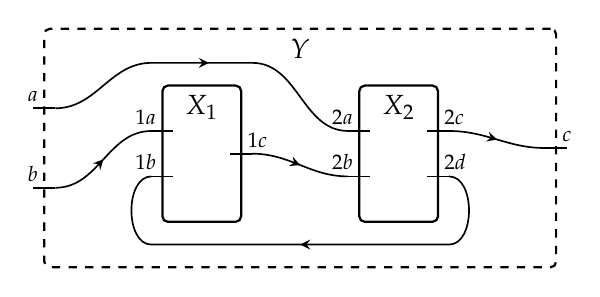
\begin{tikzpicture}[wiring diagram]
   \node[bb={2}{1}, bb name=$X_1$] (X1) {};
   \node[bb={2}{2}, right=of X1, bb name=$X_2$] (X2) {};
   \node[bb={2}{1}, dashed, fit={(X1) (X2) ($(X1.north)+(0,1.5)$) ($(X1.south)-(0,1)$)},
            bb name=$Y$] (Y) {};
   \draw[label]
      node[above left=of Y_in1]     {$a$}
      node[above left=of Y_in2]     {$b$}
      node[above right=of Y_out1]   {$c$}
      node[above left=of X1_in1]    {$1a$}
      node[above left=of X1_in2]    {$1b$}
      node[above right=of X1_out1]  {$1c$}
      node[above left=of X2_in1]    {$2a$}
      node[above left=of X2_in2]    {$2b$}
      node[above right=of X2_out1]  {$2c$}
      node[above right=of X2_out2]  {$2d$};
   \draw[ar] (Y_in2') to (X1_in1);
   \draw[ar] (X1_out1) to (X2_in2);
   \draw[ar] (X2_out1) to (Y_out1');
   \draw[ar] let \p1=(X1.north west), \p2=(X1.north east), \n1={\y1+\bby}, \n2=\bbportlen in
      (Y_in1') to (\x1-\n2,\n1) -- (\x2+\n2,\n1) to (X2_in1);
   \draw[ar] let \p1=(X2.south east), \p2=(X1.south west), \n1={\y1-\bby}, \n2=\bbportlen in
      (X2_out2) to[in=0] (\x1+\n2,\n1) -- (\x2-\n2,\n1) to[out=180] (X1_in2);
\end{tikzpicture}
\end{equation}
represent compositions. That is, new morphisms are constructed from old by specifying which outputs
will be fed back into which inputs. In fact, these are related to Penrose diagrams in $\ncat{Vect}$, and the word \emph{traced} originates in
this vector space terminology~\cite{JoyalStreetVerity}.

\section{Traced string diagrams as cobordisms}

A string diagram usually does not explicitly include the outer box $Y$. If we include it, as in
(\ref{dia:string_diagram}), the resulting \emph{wiring diagram} can be given another interpretation:
it represents a 1-dimensional cobordism between oriented 0-manifolds. For example, the box $X_1$ in
the picture includes only the data of a pair of finite sets,
$(\inp{X_1},\outp{X_1})=(\{1a,1b\},\{1c\})$, which can be interpreted as an oriented 0-manifold.
Moreover, the wiring diagram itself, in which boxes $X_1,\ldots,X_n$ are wired together inside a
larger box $Y$, can be interpreted as an oriented cobordism from $X_1\sqcup\cdots\sqcup X_n$ to $Y$.
This is a morphism in the (colored) operad $\Cob$, underlying the symmetric monoidal category of
oriented 1-cobordisms; see Section~\ref{sec:wds_and_cob}.

There is actually a bit more data in a string (or wiring) diagram for a traced category $\cat{C}$ than in a cobordism.
Namely, each input and output of a box must be labeled by an object of $\cat{C}$ and the wires connecting boxes must respect the labels (e.g., in (\ref{dia:string_diagram}) object 2d must equal object 1b). We will thus consider the operad $\LCob{\cat{O}}$ of oriented 1-dimensional cobordisms over a fixed set of
labels $\cat{O}$.

In the table below, we record these two interpretations of a string diagram. Note the ``degree
shift'' between the second and third columns.
\begin{center}
\begin{tabular}{lll}
   \toprule
      \multicolumn{3}{c}{Interpretations of string diagrams} \\
   \midrule
      String diagram & Traced category $\cat{C}$ & $\LCob{\cat{O}}$ \\
   \midrule
      Wire label set, $\cat{O}$ & Objects, $\cat{O}\coloneqq\Ob(\cat{C})$ & Label set, $\cat{O}$ \\
      Boxes, e.g., \tikz[wiring diagram,bb port sep=1,bby=2.4pt,bb min width=5.5pt,
                  bb port length=2pt,bb rounded corners=1pt,baseline=(B.south)]
               {\node[bb={1}{2}] (B) {};}
         & Morphisms in $\cat{C}$& Objects (oriented 0-mfds over $\cat{O}$) \\
      String diagrams & Compositions in $\cat{C}$& Morphisms (cobordisms over $\cat{O}$) \\
      Nesting & Axioms of traced cats & Composition (of cobordisms) \\
   \bottomrule
\end{tabular}
\end{center}

\subsection{The formal connection between Cob-algebras and Traced categories}
   \label{sec:statement_of_main_thm}

The relationship between these interpretations of string diagrams is most easily made precise when
the set $\cat{O}$ of labels is fixed. Let $\TTrCat$ denote the 2-category of traced categories,
strong traced functors, and monoidal natural isomorphisms \cite{HK}, and let $\TrCat$ denote its underlying 1-category.%
\footnote{
We use a similar notational convention throughout this paper. We denote named 1-categories, monoidal categories, and operads with bold roman letters, e.g., $\ncat{Cob}$, and unnamed 1-categories with script, e.g., $\cat{C}$. For named 2-categories or bicategories we do almost the same, but change the font of the first letter to calligraphic, such as $\nncat{T}{rCat}$; for unnamed 2-categories we use (unbold) calligraphic, e.g., $\ccat{D}$. Finally, for double categories we make the first letter  blackboard bold, whether named (e.g., $\ndcat{P}{rof}$) or unnamed (e.g., $\dcat{D}$).
}
Finally, let $\TrCat_{\cat{O}}$ denote the subcategory in which the object set is fixed to be free on the set $\cat{O}$---which we
call its label set---together with label-preserving maps. For any monoidal category
$\cat{M}$, we denote by $\cat{M}\alg=\ncat{Lax}(M,\Set)$ the category of lax functors $\cat{M}\to\Set$. Then there
is an equivalence of categories
\begin{equation}\label{eq:single_fiber}
   \LCob{\cat{O}}\alg\simeq\TrCat_{\cat{O}}.
\end{equation}
Some intuition for this statement will be given in Section~\ref{subsec:cobalg_and_trCat}, and it will be generalized in \ref{thm:Theorem_A} and proven as such in Section~\ref{sec:proof_of_A}.
\subsection{The main results}\label{subsec:main_results}

The equivalence (\ref{eq:single_fiber}) has two drawbacks: the object set of the traced category is fixed, and it is assumed to be free. Much of the work in this paper is to relax these two conditions. For the latter, we prove that the 2-category of traced categories is equivalent to that of \emph{object-free} traced categories (see Proposition~\ref{prop:TrCat_ObjectFree}). For the former, we first explain what kind of variance is appropriate.

A strong functor $F\colon T\to T'$ between object-free traced categories sends each object in $T$ to the tensor product of finitely many objects in $T'$; that is, it induces a function $\Ob F\colon\Ob T\to\List(\Ob T')$, where $\List\colon\Set\to\Set$ is the free monoid monad. Let $\ncat{Kls}$ denote the Kleisli category of this monad, so $\Ob F$ is identified with a morphism in $\ncat{Kls}$. By Lemma~\ref{lemma:monad_morphism}, there is a functor $(\LCob{\bullet})\colon\ncat{Kls}\to\CompCat$, \todo{Patrick: check this paragraph; is $(\LCob{\bullet})$ clear enough notation?}and we can compose it with $\Lax(-,\Set)$ to obtain a functor which we denote
\begin{equation}\label{eqn:cob/bullet}
(\LCob{\bullet})\alg\colon\op{\ncat{Kls}}\too\Cat.
\end{equation}
By applying the Grothendieck construction to (\ref{eqn:cob/bullet}), we collect the equivalences (\ref{eq:single_fiber}) for varying $\cat{O}$ into a single functor, and we have the following main result, whose proof can be found in Section~\ref{sec:proof_of_A}.

\begin{named}{Theorem A}\label{thm:Theorem_A}
   There is a fully-faithful functor of 1-categories
   \begin{equation*}
      \CobKlsAlg \to \TrCat
   \end{equation*}
   such that the induced 2-functor $\CobKlsAlg\to\TTrCat$ is 2-essentially surjective.
\end{named}

\section{Generalization: Lax algebras on compact categories}

It is most convenient to prove~\ref{thm:Theorem_A} by proving a more general result, which
gives an equivalence between the category of lax functors out of any compact category $\cat{C}$ and the category of
strong, bijective-on-objects functors out of $\cat{C}$,
\begin{equation}\label{eqn:lax_compcat_bo}
\Lax(\cat{C},\Set)\iso\cat{C}/\CompCat^{\bo}.
\end{equation}
As in Section~\ref{subsec:main_results}, the difficulty is allowing this equivalence to vary appropriately with $\cat{C}$.

The definition of compact closed symmetric
monoidal category, hereafter \emph{compact category}, can be found in Section~\ref{sec:compact_and_int}, or in~\cite{MacLane}. Let $\CompCat$ denote the category of compact categories and strong
monoidal functors between them. We show in Lemma~\ref{lemma:factorization_system} that there is a
factorization system on $\CompCat$, in which the left class consists of bijective-on-objects
functors and the right class consists of fully faithful functors. Let $\CompCat^{\bo}$ be the full
subcategory of the arrow category $\CompCat^{\to}$ spanned by the bijective-on-objects functors.

\begin{named}{Theorem B}\label{thm:TheoremB}
   There is an equivalence of fibrations
   \begin{equation*}
      \begin{tikzcd}[column sep=0em]
         \int^{\cat{C}\in\CompCat}\Lax(\cat{C},\Set) \ar[rr,"\equiv"] \ar[dr,two heads]
            && \CompCat^{\bo} \ar[dl,two heads,"\dom"] \\
            & \CompCat &
      \end{tikzcd}
   \end{equation*}
\end{named}

Recall from~\cite{JoyalStreetVerity} that traced categories are full subcategories of compact
categories. The Int construction, applied to a traced category $\cat{C}$, returns the smallest
compact category $\Int(\cat{C})$ of which it is a subcategory; we call $\Int(\cat{C})$ the
\emph{compact closure} of $\cat{C}$. We will recall these notions in Sections~\ref{sec:intuition_for_traced}~and~\ref{sec:compact_and_int}.

It turns out that if our compact category $\cat{C}$ is the compact closure of some traced category
$\cat{D}$, then~\ref{thm:TheoremB} lifts to a result about $\cat{D}$. We record this result
as~\ref{cor:CorollaryB}, from which~\ref{thm:Theorem_A} follows. These are proved in
Section~\ref{sec:generalization}.

\begin{named}{Corollary B}\label{cor:CorollaryB}
   There is an equivalence of fibrations
   \begin{equation*}
      \begin{tikzcd}[column sep=0em]
         \int^{\cat{C}\in\TrCat}\Lax(\Int(\cat{C}),\Set) \ar[rr,"\equiv"] \ar[dr,two heads]
            && \TrCat^{\bo} \ar[dl,two heads,"\dom"] \\
            & \TrCat &
      \end{tikzcd}
   \end{equation*}
\end{named}


\section{Wiring Diagrams, cobordisms, and traced categories}

In this section, we give a bit more intuition about the connection between wiring diagrams and cobordisms, and the equivalence between the category of traced categories
and the category of cobordism algebras.

\subsection{Wiring diagrams and $\Cob$}\label{sec:wds_and_cob}

The objects in $\Cob$ are signed sets $(\inp{X},\outp{X})$, each of which can be drawn as a box with
input wires $\inp{X}$ drawn entering the box, on its left, and output wires $\outp{X}$ drawn exiting
the box, on its right. We call the latter style \emph{an interface}.

\[
   \begin{tikzpicture}[node distance=0 and 0, baseline=(current bounding box.center)]
      \node (A1) {$-$};
      \node[below=-.1 of A1] (A2) {$-$};
      \node[below=-.1 of A2] (A3) {$-$};
      \node[below=-.1 of A3] (B1) {$+$};
      \node[below=-.1 of B1] (B2) {$+$};
   \end{tikzpicture}
   \hspace{4em}
   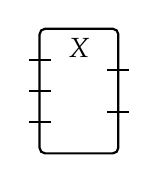
\begin{tikzpicture}[wiring diagram, bby=1.2ex, baseline=(current bounding box.center)]
      \node[bb={3}{2},bb name=$X$] {};
   \end{tikzpicture}
\]

Wiring diagrams seem to be a new way to visualize morphisms in the symmetric monoidal category
$\Cob$ of 1-dimensional oriented cobordisms. In fact, they are better suited to the operad associated to $\Cob$. The following shows the two approaches to drawing a 2-ary morphism $X_1,X_2\to Y$:

\[
   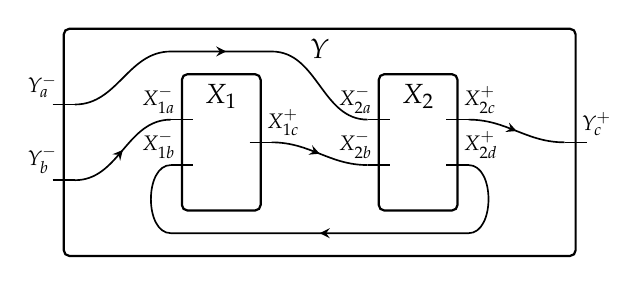
\begin{tikzpicture}[wiring diagram, baseline=(current bounding box.center)]
      \node[bb={2}{1}, bb name=$X_1$] (X1) {};
      \node[bb={2}{2}, right=of X1, bb name=$X_2$] (X2) {};
      \node[bb={2}{1}, fit={(X1) (X2) ($(X1.north)+(0,1)$) ($(X1.south)-(0,1)$)},bb name =$Y$] (Y) {};
      \draw[label]
          node[above left=of Y_in1]     {$\inp{Y}_a$}
          node[above left=of Y_in2]     {$\inp{Y}_b$}
          node[above right=of Y_out1]   {$\outp{Y}_c$}
          node[above left=of X1_in1]    {$\inp{X}_{1a}$}
          node[above left=of X1_in2]    {$\inp{X}_{1b}$}
          node[above right=of X1_out1]  {$\outp{X}_{1c}$}
          node[above left=2pt and -2pt of X2_in1]    {$\inp{X}_{2a}$}
          node[above left=of X2_in2]    {$\inp{X}_{2b}$}
          node[above right=of X2_out1]  {$\outp{X}_{2c}$}
          node[above right=of X2_out2]  {$\outp{X}_{2d}$};
      \draw[ar] (Y_in2') to (X1_in1);
      \draw[ar] (X1_out1) to (X2_in2);
      \draw[ar] (X2_out1) to (Y_out1');
      \draw[ar] let \p1=(X1.north west), \p2=(X1.north east), \n1={\y1+\bby}, \n2=\bbportlen in
          (Y_in1') to (\x1-\n2,\n1) -- (\x2+\n2,\n1) to (X2_in1);
      \draw[ar] let \p1=(X2.south east), \p2=(X1.south west), \n1={\y1-\bby}, \n2=\bbportlen in
         (X2_out2) to[in=0] (\x1+\n2,\n1) -- (\x2-\n2,\n1) to[out=180] (X1_in2);
   \end{tikzpicture}
   \qquad
   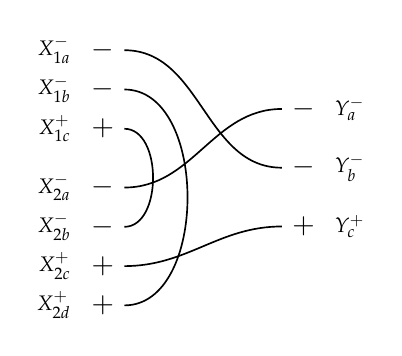
\begin{tikzpicture}[x=1cm,y=1ex,node distance=1 and 1,semithick,every label quotes/.style={font=\everymath\expandafter{\the\everymath\scriptstyle}},every to/.style={out=0,in=180},baseline=(current bounding box.center)]
      \node ["$\inp{X}_{1a}$" left] (X1a) {$-$};
      \node [below=0 of X1a, "$\inp{X}_{1b}$" left] (X1b) {$-$};
      \node [below=0 of X1b, "$\outp{X}_{1c}$" left] (X1c) {$+$};
      \node [below=1.5 of X1c, "$\inp{X}_{2a}$" left] (X2a) {$-$};
      \node [below=0 of X2a, "$\inp{X}_{2b}$" left] (X2b) {$-$};
      \node [below=0 of X2b, "$\outp{X}_{2c}$" left] (X2c) {$+$};
      \node [below=0 of X2c, "$\outp{X}_{2d}$" left] (X2d) {$+$};
      \node [below right=1.5 and 2 of X1a, "$\inp{Y}_a$" right] (Ya) {$-$};
      \node [below=1.5 of Ya, "$\inp{Y}_b$" right] (Yb) {$-$};
      \node [below=1.5 of Yb, "$\outp{Y}_c$" right] (Yc) {$+$};
      \draw (X1a) to (Yb);
      \draw (X1b) to[in=0] (X2d);
      \draw (X1c) to[in=0] (X2b);
      \draw (X2a) to (Ya);
      \draw (X2c) to (Yc);
   \end{tikzpicture}
\]

\subsection{$\Cob$-algebras and traced categories}\label{subsec:cobalg_and_trCat}

Here we sketch the equivalence of categories 
$$\LCob{\cat{O}}\alg\simeq\TrCat_{\cat{O}}$$
from Section~\ref{sec:statement_of_main_thm}. We will see that the same data are required, and the same conditions are
satisfied, whether one is specifying a lax functor $P\in\LCob{\cat{O}}\alg$ or a traced category
$\cat{C}\in\TrCat_{\cat{O}}$ with objects generated by $\cat{O}$. 

First, for each box $X=(\inp{X},\outp{X})$ that might appear in a string diagram, both $P\colon\LCob{\cat{O}}\to\Set$ and
$\cat{C}$ require a set, $P(X)$ and $\Hom_{\cat{C}}(\inp{X},\outp{X})$, respectively.
Second, for each string diagram, both $P$ and $\cat{C}$ require a function: an action on morphisms,
in the case of $P$, and a formula for performing the required compositions, tensors, and traces, in
the case of $\cat{C}$. The condition that $P$ is functorial corresponds to the fact that $\cat{C}$
satisfies the axioms of traced categories. 

We will briefly specifying how to construct a lax functor $P$ from a traced category $(\cat{C},\otimes,I,\Tr)$, whose objects are freely generated by $\cat{O}$. We will abuse notation slightly as follows: Given a relative set
$\iota\colon Z\to\cat{O}$, we will use the same symbol $Z$ to denote
the tensor $\bigotimes_{z\in Z}\iota(z)$ in $\cat{C}$. 

For an oriented 0-manifold $X=\inp{X}\sqcup \outp{X}$ over $\cat{O}$, we
set $P(X)\coloneqq\Hom_{\cat{C}}(\inp{X},\outp{X})$. Given a cobordism $\Phi\colon X\to Y$, we need a function $P(\Phi)\colon P(X)\to P(Y)$. For any cobordism $\Phi$, there exist
$A,B,C,D,E\in\Ob\cat{C}$ such that $\inp{X}\cong C\otimes A$, $\outp{X}\cong C\otimes B$,
$\inp{Y}\cong A\otimes D$, $\outp{Y}\cong B\otimes D$, and $E$ is the set of floating loops in $\Phi$;
thus $\Phi$ is essentially equivalent to the cobordism shown on the right side of (\ref{eq:cob_and_trace_pic}).
\begin{equation}\label{eq:cob_and_trace_pic}
   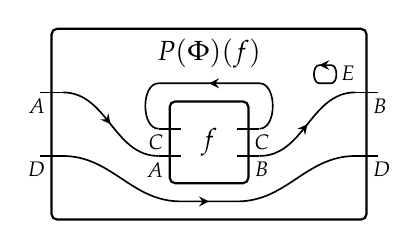
\begin{tikzpicture}[wiring diagram, bby=1.4ex, baseline=(current bounding box.center)]
      \node[bb port sep=1.5, bb={2}{2}] (domain) {$f$};
      \node[bb={2}{2}, fit={(domain) ($(domain.north)+(0,3)$) ($(domain.south)-(0,1)$)}, bb name=$P(\Phi)(f)$] (codomain) {};
      \draw[ar] (codomain_in1') to (domain_in2);
      \draw[ar] (domain_out2) to (codomain_out1');
      \draw[ar] let \p1=(domain.north east), \p2=(domain.north west), \n1={\y1+\bby}, \n2=\bbportlen in
          (domain_out1) to[in=0] (\x1+\n2,\n1) -- (\x2-\n2,\n1) to[out=180] (domain_in1);  %Trace on C
      \draw[ar] let \p1=(domain.south west), \p2=(domain.south east), \n1={\y1-\bby}, \n2=\bbportlen in
          (codomain_in2') to[in=180] (\x1+\n2,\n1) -- (\x2-\n2,\n1) to[out=0] (codomain_out2'); %Identity on D
      \draw[ar] let \p1=(domain.north east) in
          (\x1+.7*\bbx,\y1+\bby) to[in=0] (\x1+.7*\bbx,\y1+2*\bby) -- (\x1+.6*\bbx,\y1+2*\bby) to[out=180] (\x1+.6*\bbx,\y1+\bby) -- (\x1+.7*\bbx,\y1+\bby);%Loop
      \draw[label] let \p1=(domain.north east) in
          node[below left=of codomain_in1]     {$A$}
          node[below left=of codomain_in2]     {$D$}
          node[below right=of codomain_out1]    {$B$}
          node[below right=of codomain_out2]    {$D$}
          node[above left=.6 and 0 of codomain_out1']  {$E$}
          node[below left=of domain_in1]     {$C$}
          node[below left=of domain_in2]     {$A$}
          node[below right=of domain_out2]    {$B$}
          node[below right=of domain_out1]   {$C$};
   \end{tikzpicture}
   \qquad\qquad
   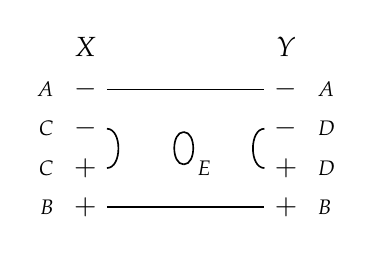
\begin{tikzpicture}[x=1cm,y=1ex,node distance=1 and 1,semithick,every label quotes/.style={font=\everymath\expandafter{\the\everymath\scriptstyle}},every to/.style={out=0,in=180},baseline=(current bounding box.center)]
      \node ["$A$" left] (X1a) {$-$};
      \node [above=0.25 of X1a] {$X$};
      \node [below=0 of X1a, "$C$" left] (X1b) {$-$};
      \node [below=0 of X1b, "$C$" left] (X2a) {$+$};
      \node [below=0 of X2a, "$B$" left] (X2b) {$+$};
      \node [right=2 of X1a, "$A$" right] (Y1a) {$-$};
      \node [above=0.25 of Y1a] {$Y$};
      \node [below=0 of Y1a, "$D$" right] (Y1b) {$-$};
      \node [below=0 of Y1b, "$D$" right] (Y2a) {$+$};
      \node [below=0 of Y2a, "$B$" right] (Y2b) {$+$};
      \node [right=1.45 of X2a, "$E$" left] {};
      \draw (X1a) to (Y1a);
      \draw (X1b) to[in=0] (X2a);
      \draw (X2b) to (Y2b);
      \draw (Y1b) to[in=180,out=180] (Y2a);
      \draw ($(X1b)+(1.25,-2.75)$) to[in=0] ($(X1b)+(1.25,-0.25)$);
      \draw ($(X1b)+(1.25,-0.25)$) to[in=180,out=180] ($(X1b)+(1.25,-2.75)$);
   \end{tikzpicture}
\end{equation}
With the above notation, for $f\in P(X)$ we can follow the string diagram (left of (\ref{eq:cob_and_trace_pic})) and define
\begin{equation}\label{eq:cob algebra formula}
   P(\Phi)(f)\coloneqq\Tr_{A,B}^C(f)\otimes D\otimes\Tr^E_{I,I}(\id_E).
\end{equation}


\section{Applications of the operadic perspective}

The operadic perspective on traced categories may be useful in concrete applications, such as for
modeling nested process diagrams. It may also be useful in pure mathematics, because the operad $\Cob$,
which indexes traced categories, can be easily modified to model a variety of other doctrines.
These two applications will be discussed in more detail in
Sections~\ref{sec:modular}~and~\ref{sec:math application} respectively.

\subsection{Modular design}\label{sec:modular}

When designing or investigating a complex system, it is often useful to think in terms of
interacting subsystems, put together to make a larger whole. In manufacturing, this is often called
\emph{modular design}. Each object in $\Cob$ represents an interface, or \emph{module}, with a
fixed number and type of inputs and outputs. The morphisms in $\Cob$ correspond to strategies by
which these interfaces can be wired together into a process, which itself has an interface.

An algebra $P\colon\Cob\to\Set$ provides semantics for these boxes (\cite{RupelSpivak},\cite{VagnerSpivakLerman}). For each interface $X$, the set
$P(X)$ represents the set of ``fillers'' for this interface. For example, one might imagine that
each interface $X$ can be filled by any state machine having that interface; in this case $P(X)$ is
the set of such state machines. For a morphism $\varphi\colon X_1,\ldots,X_n\to Y$, the function
$P(\varphi)$ tells us how to construct a filler of type $Y$, given fillers on each $X_i$.
Composition of cobordisms are drawn as nested diagrams:

\[
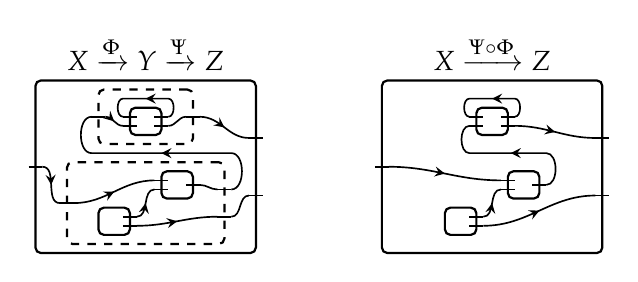
\begin{tikzpicture}[wiring diagram, bb small]
   \node[bb={2}{2}] (X1) {};
   \node[bb={1}{1}, fit={(X1) ($(X1.north)+(0,1)$)}, dashed] (Y1) {};
   \node[bb={2}{1}, below right=4 and 0 of X1] (X2) {};
   \node[bb={0}{2},below left=of X2] (X3) {};
   \node[bb={1}{2}, fit=(X2) (X3), dashed] (Y2) {};
   \node[bb={1}{2}, fit=(Y1) (Y2)] (Z) {};
   \draw[ar] (Z_in1') to (Y2_in1);
   \draw[ar] (Y2_in1') to (X2_in1);
   \draw[ar] (X3_out1) to (X2_in2);
   \draw[ar] (X3_out2) to (Y2_out2');
   \draw (Y2_out2) to (Z_out2');
   \draw[ar] (Y1_in1') to (X1_in2);
   \draw (X1_out2) to (Y1_out1');
   \draw[ar] (Y1_out1) to (Z_out1');
   \draw (X2_out1) to (Y2_out1');
   \draw[ar] let \p1=(Y2.north east), \p2=(Y1.south west), \n1={\y1+\bby}, \n2=\bbportlen in
      (Y2_out1) to[in=0] (\x1+\n2,\n1) -- (\x2-\n2,\n1) to[out=180] (Y1_in1);
   \draw[ar] let \p1=(X1.north east), \p2=(X1.north west), \n1={\y1+\bby}, \n2=\bbportlen in
      (X1_out1) to[in=0] (\x1+\n2,\n1) -- (\x2-\n2,\n1) to[out=180] (X1_in1);
   \node[anchor=south] at (Z.north) {$X\xrightarrow{\Phi}Y\xrightarrow{\Psi}Z$};

   \node[bb={2}{2}, right=10 of X1] (X1') {};
   \node[bb={2}{1}, below right=4 and 0 of X1'] (X2') {};
   \node[bb={0}{2},below left=of X2'] (X3') {};
   \node[bb={1}{2}, fit={($(X1'.north)+(0,1)$) (X2') (X3')}, inner xsep=2*\bbx, inner ysep=2*\bby] (Z') {};
   \draw[ar] (X3'_out1) to (X2'_in2);
   \draw[ar] (Z'_in1') to (X2'_in1);
   \draw[ar] (X1'_out2) to (Z'_out1');
   \draw[ar] (X3'_out2) to (Z'_out2');
   \draw[ar] let \p1=(X2'.north east), \p2=(X1'.south west), \n1={\y1+2*\bby}, \n2=\bbportlen in
      (X2'_out1) to[in=0] (\x1+\n2,\n1) -- (\x2-\n2,\n1) to[out=180] (X1'_in2);
   \draw[ar] let \p1=(X1'.north east), \p2=(X1'.north west), \n1={\y1+\bby}, \n2=\bbportlen in
      (X1'_out1) to[in=0] (\x1+\n2,\n1) -- (\x2-\n2,\n1) to[out=180] (X1'_in1);
   \node[anchor=south] at (Z'.north) {$X\xrightarrow{\Psi\circ\Phi}Z$};
\end{tikzpicture}
\]

In our model for modular design, any way to chunk the small boxes inside the big one will yield the
same result. This is a reflection of the functoriality of $P\colon\Cob\to\Set$, which says that
commutative diagrams in $\Cob$ are sent to commutative diagrams of sets. Nested structures, given
by composition of such morphisms, may be useful for the kind of chunking that humans use to
understand complex systems~\cite{Miller}.

\subsection{Mathematical application: varying the operad}\label{sec:math application}

Formalizing modular design using operads, as in~\cite{Spivak},~\cite{RupelSpivak}, and~\cite{VagnerSpivakLerman} was the original
motivation for the present paper, as the drawings had strong similarities to those found in traced
categories. However, it should be noted that none of these papers actually uses $\Cob$ as the
indexing category for their algebras. In fact, they use three different operads, of varying degrees
of similarity to $\Cob$. For example, there is an orthogonal factorization system on $\Cob$, for
which morphisms in the left class $\cat{L}$ include no closed loops, and the operad of interest in~\cite{VagnerSpivakLerman} is $\cat{L}$.

If one wished to make minor modifications in the axioms of traced categories to create some new sort of category $\ncat{Tr'Cat}$, one may proceed by imagining the string diagrams make sense in $\ncat{Tr'Cat}$. For example, one may want to consider cartesian traced categories, in which wires can split or terminate abruptly. Or they may want to allow splitting but not allow abrupt termination. 
\begin{center}
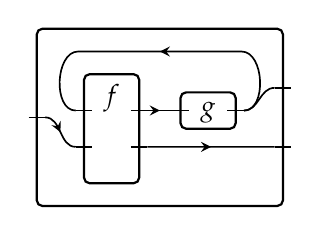
\begin{tikzpicture}[wiring diagram,bb min width =.7cm, bb port sep =1, bbx=.6cm,bb port length=3pt]
   \node[bb port sep=1.6, bb={2}{2}, bb name=$f$] (X1) {};
   \node[bb port sep=.8,bb={1}{1}, right=.7 of X1_out1, bb name=$g$] (X2) {};
   \node[bb={1}{2}, fit={(X1) (X2) ($(X1.north)+(0,1)$)}] (Y) {};
   \draw[ar] (Y_in1') to (X1_in2);
   \draw[ar,pos=.8] (X1_out1) to (X2_in1);
   \draw (X2_out1) to (Y_out1');
   \draw[ar] (X1_out2) to (Y_out2');
   \draw[ar] let \p1=(X2.north east), \p2=(X1.north west), \n1={\y2+\bby}, \n2=\bbportlen in
      (X2_out1) to[in=0] (\x1+.7*\n2,\n1) -- (\x2-.7*\n2,\n1) to[out=180] (X1_in1);
\end{tikzpicture}
\end{center}
We can accommodate the desired notion of string diagrams for $\ncat{Tr'Cat}$ by modifying the indexing operad $\Cob$ to some $\Cob'$. Using $\cat{L}$ for dynamical systems in \cite{VagnerSpivakLerman} is an example of this. As another, suppose that, as above, we want string diagrams in which wires can split but not terminate. Noting that an oriented cobordism $\varphi$ includes the data of a function
$$\varphi_1\colon\inp{X}\sqcup\outp{Y}\to\outp{X}\sqcup\inp{Y},$$ 
which is both injective and surjective, we can obtain the desired indexing operad $\Cob'$ by requiring surjectivity but not injectivity in $\varphi$.


\section{Plan of the paper} \todo{This plan needs work!}

The paper is organized as follows. In Section~\ref{sec:traced categories} we give more details on
the connection between traced monoidal categories, their string diagrams, and algebras on the operad
of cobordisms. In Section~\ref{sec:generalization} we prove~\ref{thm:TheoremB}
and~\ref{cor:CorollaryB}, which compare lax set-valued functors to strong bijective-on-objects
functors, respectively for compact and traced categories. Our main result,~\ref{thm:Theorem_A},
which says that traced categories are $\Cob$-algebras, follows easily.

\section*{Acknowledgments}

Thanks go to Steve Awodey and Ed Morehouse for suggesting we formally connect the operad-algebra
picture in \cite{RupelSpivak} to string diagrams in traced categories.

\chapter{Categorical preliminaries}\label{sec:traced categories}

In this section we remind the reader of some categorical preliminaries. Basic definitions and facts
about monoidal, traced, and compact categories, lax and strong functors, and the Int construction
are given in Sections~\ref{sec:prelim monoidal}~through~\ref{sec:compact_and_int}. The fact that
the free compact category on a set has an algebraic description in terms of bijections between
signed sets, and the fact that it has a geometric description in terms of 1-dimensional oriented
cobordisms is recalled in Section~\ref{sec:free and geometry}. 

\section{Monoidal categories}\label{sec:prelim monoidal}

Let $\cat{C}$ and $\cat{D}$ be monoidal categories. Recall that a functor
$F\colon\cat{C}\to\cat{D}$ is called \emph{lax monoidal} if it is equipped with a morphism
\[
\begin{tikzcd}
   I_D \rar{\epsilon} & F(I_C)
\end{tikzcd}
\]
and a natural transformation
\[
\begin{tikzcd}
   F(X) \otimes_D F(Y) \rar{\mu_{X,Y}} & F(X\otimes_C Y)
\end{tikzcd}
\]
such that for all $X,Y,Z\in\cat{C}$, the diagram (suppressing associators)
\[
\begin{tikzcd}
   F(X)\otimes F(Y) \otimes F(Z)
      \rar{\id\otimes\mu}
      \dar[swap]{\mu\otimes\id}
   & F(X)\otimes F(Y\otimes Z)
      \dar{\mu} \\
   F(X\otimes Y)\otimes F(Z)
      \rar[swap]{\mu}
   & F(X\otimes Y\otimes Z)
\end{tikzcd}
\]
commutes, and for all $X\in\cat{C}$ the two diagrams
\[
\begin{tikzcd}
   I_D\otimes F(X)
      \dar[swap]{\epsilon\otimes\id}
   & F(X)
      \lar[swap]{l_{F(X)}}
      \dar{F(l_X)} \\
   F(I_C)\otimes F(X)
      \rar[swap]{\mu}
   & F(I_C\otimes X)
\end{tikzcd}
\qquad
\begin{tikzcd}
   F(X) \otimes I_D
      \dar[swap]{\id\otimes\epsilon}
   & F(X)
      \lar[swap]{r_{F(X)}}
      \dar{F(r_X)} \\
   F(X)\otimes F(I_C)
      \rar[swap]{\mu}
   & F(X\otimes I_C)
\end{tikzcd}
\]
commute.
If $\epsilon$ and $\mu$ are isomorphisms, then $F$ is \emph{strong}.

If $\cat{C}$ and $\cat{D}$ are symmetric monoidal, then $F$ is a \emph{lax symmetric monoidal
functor} if it is lax monoidal, and commutes with the symmetries, in the sense that the diagram
\[
\begin{tikzcd}
   F(X)\otimes F(Y)
      \rar{\sigma}
      \dar[swap]{\mu}
   & F(Y)\otimes F(X)
      \dar{\mu} \\
   F(X\otimes Y)
      \rar[swap]{F(\sigma)}
   & F(Y\otimes X)
\end{tikzcd}
\]
commutes.

If $F$ and $G$ are lax monoidal functors (possibly symmetric), then a natural transformation
$\alpha\colon F\to G$ is called a \emph{monoidal transformation} if the diagrams
\[
\begin{tikzcd}
   F(X)\otimes F(Y)
      \rar{\alpha_X\otimes\alpha_Y}
      \dar[swap]{\mu}
   & G(X)\otimes G(Y)
      \dar{\mu} \\
   F(X\otimes Y)
      \rar[swap]{\alpha_{X\otimes Y}}
   & G(X\otimes Y)
\end{tikzcd}
\qquad
\begin{tikzcd}[column sep=tiny]
   {} & I_D \dlar[swap]{\epsilon} \drar{\epsilon} & \\
   F(I_C) \ar{rr}[swap]{\alpha_I} && G(I_C)
\end{tikzcd}
\]
commute.

Let $\MMonCat$ denote the 2-category of symmetric monoidal categories, strong monoidal functors, and
monoidal transformations, and let $\MonCat$ denote the underlying 1-category. Let
$\Lax(\cat{C},\cat{D})$ denote the category of lax monoidal functors and monoidal transformations
from $\cat{C}$ to $\cat{D}$. Whenever we discuss monoidal categories in this paper will mean symmetric monoidal.

\section{Traced categories}\label{sec:intuition_for_traced}

A trace on a (symmetric) monoidal category is a collection of functions
\begin{equation}\label{dia:trace function}
   \Tr^U_{X,Y}\colon\Hom(U\otimes X,U\otimes Y)\to\Hom(X,Y)
\end{equation}
for $U,X,Y\in\Ob(\cat{M})$ satisfying several, say six, axioms. When traced categories are defined, one often
sees the trace functions, as well as each of the axioms, accompanied by a picture. For example,
(\ref{dia:trace function}) applied to an arbitrary $f\colon U\otimes X\to U\otimes Y$ might be
accompanied by this picture:
$$
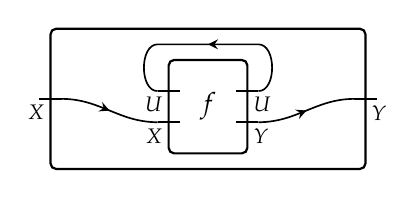
\begin{tikzpicture}[wiring diagram,bby=1.2ex]
   \node[bb={2}{2}] (domain) {$f$};
   \node[bb={1}{1}, fit={(domain) ($(domain.north)+(0,1)$)}] (codomain) {};
   \draw[ar] (codomain_in1') to (domain_in2);
   \draw[ar] (domain_out2) to (codomain_out1');
   \draw[ar] let \p1=(domain.north east), \p2=(domain.north west), \n1={\y1+\bby}, \n2=\bbportlen in
      (domain_out1) to[in=0] (\x1+\n2,\n1) -- (\x2-\n2,\n1) to[out=180] (domain_in1);
   \draw[label]
       node[below left=of codomain_in1]     {$X$}
       node[below right=of codomain_out1]    {$Y$}
       node[below left=of domain_in1]     {$U$}
       node[below left=of domain_in2]     {$X$}
       node[below right=of domain_out2]    {$Y$}
       node[below right=of domain_out1]   {$U$};
\end{tikzpicture}
$$
This can be recognized as a cobordism between oriented 0-manifolds, as we discussed in
Section~\ref{sec:wds_and_cob}. Each of the six axioms is vacuous from this perspective, in
the sense that both sides of the equation correspond to the same cobordism. For example, here are
the axioms of \emph{dinaturality} and \emph{superposition}:
\begin{itemize}
   \item For every $f\colon U\otimes X\to V\otimes Y$ and $g:V\to U$ we have
      \[
         \Tr^U_{X,Y}\Big[\big(g\otimes Y\big)\circ f\Big]=\Tr^V_{X,Y}\Big[f\circ\big(g\otimes X\big)\Big];
      \]
      \[\tikzset{bbx=1cm}
         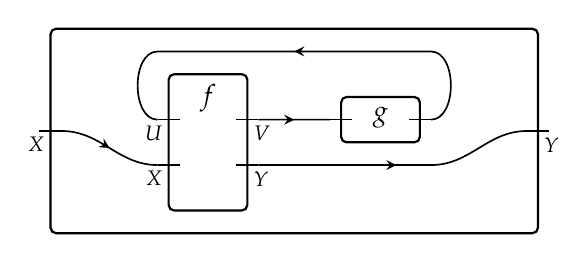
\begin{tikzpicture}[wiring diagram,baseline=(current bounding box.center)]
            \node[bb={2}{2}, bb name=$f$] (X1) {};
            \node[bb port sep=1,bb={1}{1}, right=.7 of X1_out1, bb name=$g$] (X2) {};
            \node[bb={1}{1}, fit={(X1) (X2) ($(X1.north)+(0,1)$)}] (Y) {};
            \draw[ar] (Y_in1') to (X1_in2);
            \draw[ar,pos=.8] (X1_out1) to (X2_in1);
            \draw[ar] let \p1=(X2.south east), \n1={\y1-\bby}, \n2=\bbportlen in
                (X1_out2) -- (\x1+\n2,\n1) to (Y_out1');
            \draw[ar] let \p1=(X2.north east), \p2=(X1.north west), \n1={\y2+\bby}, \n2=\bbportlen in
                  (X2_out1) to[in=0] (\x1+\n2,\n1) -- (\x2-\n2,\n1) to[out=180] (X1_in1);
            \draw[label]
                node[below left=of Y_in1]     {$X$}
                node[below right=of Y_out1]    {$Y$}
                node[below left=of X1_in1]     {$U$}
                node[below left=of X1_in2]     {$X$}
                node[below right=of X1_out2]    {$Y$}
                node[below right=of X1_out1]   {$V$};
         \end{tikzpicture}
         =
         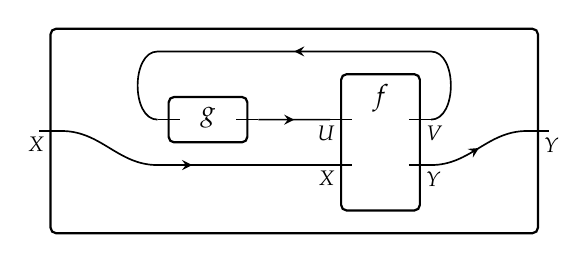
\begin{tikzpicture}[wiring diagram,baseline=(current bounding box.center)]
            \node[bb={2}{2}, bb name=$f$] (X1) {};
            \node[bb port sep=1,bb={1}{1}, left=.7 of X1_in1, bb name=$g$] (X2) {};
            \node[bb={1}{1}, fit={(X1) (X2) ($(X1.north)+(0,1)$)}] (Y) {};
            \draw[ar] let \p1=(X2.south west), \n1={\y1-\bby}, \n2=\bbportlen in
                (Y_in1') to (\x1-\n2,\n1) -- (X1_in2);
            \draw[ar] (X2_out1) to (X1_in1);
            \draw[ar] (X1_out2) to (Y_out1');
            \draw[ar] let \p1=(X1.north east), \p2=(X2.north west), \n1={\y1+\bby}, \n2=\bbportlen in
                  (X1_out1) to[in=0] (\x1+\n2,\n1) -- (\x2-\n2,\n1) to[out=180] (X2_in1);
            \draw[label]
                node[below left=of Y_in1]     {$X$}
                node[below right=of Y_out1]    {$Y$}
                node[below left=of X1_in1]     {$U$}
                node[below left=of X1_in2]     {$X$}
                node[below right=of X1_out2]    {$Y$}
                node[below right=of X1_out1]   {$V$};
         \end{tikzpicture}
         \]
   \item For every $f\colon U\otimes X\to U\otimes Y$ and $g\colon W\to Z$ we have
      \[
         \Tr^U_{X,Y}\big[f\big]\otimes g=\Tr^U_{X\otimes W,Y\otimes Z}\big[f\otimes g\big];
      \]
      \[\tikzset{bbx=.8cm,bb port sep=1.5}
      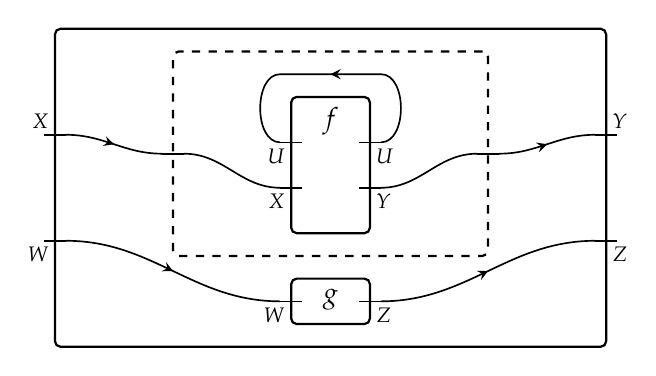
\begin{tikzpicture}[wiring diagram,baseline=(current bounding box.center)]
         \node[bb={2}{2}, bb name=$f$] (X1) {};
         \node[bb port sep=1,bb={1}{1}, below=2 of X1, bb name=$g$] (X2) {};
         \node[bb={1}{1}, fit={(X1) ($(X1.north)+(0,1)$)}, dashed] (Z) {};
         \node[bb={2}{2}, fit={(Z) (X2)}] (Y) {};
         \draw[ar] (Y_in1') to (Z_in1);
         \draw (Z_in1') to (X1_in2);
         \draw[ar] (Y_in2') to (X2_in1);
         \draw (X1_out2) to (Z_out1');
         \draw[ar] (Z_out1) to (Y_out1');
         \draw[ar] (X2_out1) to (Y_out2');
         \draw[ar] let \p1=(X1.north east), \p2=(X2.north west), \n1={\y1+\bby}, \n2=\bbportlen in
             (X1_out1) to[in=0] (\x1+\n2,\n1) -- (\x2-\n2,\n1) to[out=180] (X1_in1);
         \draw[label]
             node[above left=of Y_in1] {$X$}
             node[below left=of Y_in2] {$W$}
             node[above right=of Y_out1] {$Y$}
             node[below right=of Y_out2] {$Z$}
             node[below left=of X1_in1] {$U$}
             node[below left=of X1_in2] {$X$}
             node[below right=of X1_out2] {$Y$}
             node[below right=of X1_out1] {$U$}
             node[below left=of X2_in1] {$W$}
             node[below right=of X2_out1] {$Z$};
      \end{tikzpicture}
      =
      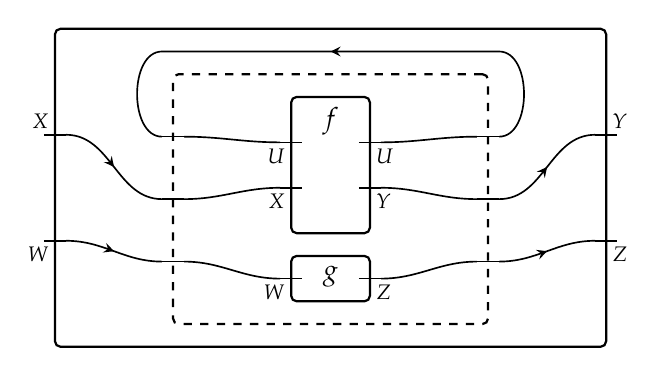
\begin{tikzpicture}[wiring diagram,baseline=(current bounding box.center)]
         \node[bb={2}{2}, bb name=$f$] (X1) {};
         \node[bb port sep=1,bb={1}{1}, below=of X1, bb name=$g$] (X2) {};
         \node[bb={3}{3}, fit={(X1) (X2)}, dashed] (Z) {};
         \node[bb={2}{2}, fit={(Z) ($(Z.north)+(0,1)$)}] (Y) {};
         \draw[ar] (Y_in1') to (Z_in2);
         \draw (Z_in2') to (X1_in2);
         \draw[ar] (Y_in2') to (Z_in3);
         \draw (Z_in3') to (X2_in1);
         \draw (X1_out2) to (Z_out2');
         \draw[ar] (Z_out2) to (Y_out1');
         \draw (X2_out1) to (Z_out3');
         \draw[ar] (Z_out3) to (Y_out2');
         \draw (Z_in1') to (X1_in1);
         \draw (X1_out1) to (Z_out1');
         \draw[ar] let \p1=(Z.north east), \p2=(Z.north west), \n1={\y1+\bby}, \n2=\bbportlen in
             (Z_out1) to[in=0] (\x1+\n2,\n1) -- (\x2-\n2,\n1) to[out=180] (Z_in1);
         \draw[label]
             node[above left=of Y_in1] {$X$}
             node[below left=of Y_in2] {$W$}
             node[above right=of Y_out1] {$Y$}
             node[below right=of Y_out2] {$Z$}
             node[below left=of X1_in1] {$U$}
             node[below left=of X1_in2] {$X$}
             node[below right=of X1_out2] {$Y$}
             node[below right=of X1_out1] {$U$}
             node[below left=of X2_in1] {$W$}
             node[below right=of X2_out1] {$Z$};
      \end{tikzpicture}
      \]
\end{itemize}

The definition of traced categories and traced functors can be found in~\cite{JoyalStreetVerity}. However, those authors define the 2-morphisms between traced functors to be monoidal transformations, whereas this choice does not behave appropriately with their $\Int$ construction (for example $\Int$ would not be 2-functorial). A correction was made in \cite{HK}, where it was shown that the appropriate 2-morphisms between traced functors are natural \emph{isomorphisms}. We denote by $\TTrCat$ the corrected 2-category of traced categories (where 2-cells are invertible), and we denote its underlying 1-category by $\TrCat$.

\subsection{The categories $\Prop$ and $\TrProp$ of props and traced props}\label{sec:defining props}

One can think of props as symmetric monoidal categories that are free on a fixed \emph{label set}
(also known as its set of colors). Functors between props need to descend to a function between
label sets. We define a traced prop to be a traced category whose underlying symmetric monoidal
category has the structure of a prop. Thus we have defined the 1-categories $\Prop$ and $\TrProp$;
we summarize our definitions by the pullback diagram
\[
\begin{tikzcd}
   \TrProp\ar[r]\ar[d]\arrow[dr, phantom, "\lrcorner", very near start]&\TrCat_1\ar[d]\\
   \Prop\ar[r]\ar[d,"\Ob"']\arrow[dr, phantom, "\lrcorner", very near start]&\SSymMonCat_1\ar[d,"\Ob"]\\
   \Set\ar[r,"\List"']&\Set
\end{tikzcd}
\]
where $\SSymMonCat_1$ (resp. $\TrCat_1$) is the underlying 1-category of $\SSymMonCat$ (resp.\ of
$\TrCat$), and where $\List\colon\Set\to\Set$ is the free monoid monad. This definition of $\Prop$
agrees with that in~\cite{HackneyRobertson}.\todo{Check this.}


\section{Compact categories and the Int construction}\label{sec:compact_and_int}

We will denote by $\CCompCat$ the full sub-2-category of $\MMonCat$ spanned by the compact symmetric
monoidal categories (or just compact categories for short).  Recall that a compact category is a
symmetric monoidal category $(\cat{C},\otimes,I)$ with the property that for every object
$X\in\Ob\cat{C}$ there exists an object $X^*$ and morphisms $\eta_X\colon I\to X^*\otimes X$ and
$\epsilon_X\colon X\otimes X^*\to I$ such that the following diagrams commute:
\begin{equation*}
   \begin{tikzcd}[column sep=small]
      X\arrow[r,"\id_X"]\arrow[d,"\cong"'] & X \\
      X\otimes I\arrow[d,"X\otimes\eta_X"'] & I\otimes X\arrow[u,"\cong"'] \\
      X\otimes(X^*\otimes X)\arrow[r,"\cong"'] & (X\otimes X^*)\otimes X\arrow[u,"\epsilon_X\otimes X"']
   \end{tikzcd}
   \hspace{.6in}
   \begin{tikzcd}[column sep=small]
      X^*\arrow[r,"\id_{X^*}"]\arrow[d,"\cong"'] & X^*\\
      I\otimes X^*\arrow[d,"\eta_X\otimes X^*"'] & X^*\otimes I\arrow[u,"\cong"'] \\
      (X^*\otimes X)\otimes X^*\arrow[r,"\cong"'] & X^*\otimes (X\otimes X^*)\arrow[u,"X^*\otimes\epsilon_X"']
   \end{tikzcd}
\end{equation*}

Every compact category $\cat{C}$ has a canonical trace structure, defined on a morphism $f\colon
U\otimes X\to U\otimes Y$ to morally be $\epsilon_U\circ f\circ \eta_U$. More precisely, if
$s_{A,B}$ is the symmetry isomorphism, one defines
\begin{equation*}
   \Tr^U_{X,Y}[f]\coloneqq(\epsilon_U\otimes Y)\circ (s_{U^*,U}\otimes Y)\circ (U^*\otimes f)\circ (\eta_U\otimes X)
\end{equation*}
%\todo[color=yellow]{does this formula make sense as written? i.e. it doesn't seem to give a map
%$X\to Y$?}
Thus we have a functor $\UCT\colon\CCompCat\to\TTrCat$. It is shown in~\cite{JoyalStreetVerity} that
this functor is the right half of a 2-adjunction
\begin{equation}\label{dia:traced compact adjunction}
\begin{tikzcd}
   \TTrCat\arrow[r,shift left=.5ex, "\Int"]&\CCompCat\arrow[l,shift left=.5ex,"\UCT"]
\end{tikzcd}
\end{equation}
the left half of which we describe now describe.

For a traced category $\cat{M}$ let $\widetilde{\cat{M}}=\Int(\cat{M})$ denote the category with
objects given by pairs $(\inp{X},\outp{X})$ where $\inp{X},\outp{X}\in \Ob(\cat{M})$ and morphisms
given by
\[
   \Hom_{\widetilde{\cat{M}}}\big((\inp{X},\outp{X}),(\inp{Y},\outp{Y})\big)=\Hom_{\cat{M}}(\inp{X}\otimes \outp{Y},\outp{X}\otimes \inp{Y}).
\]
For morphisms $\Phi:(\inp{X},\outp{X})\to(\inp{Y},\outp{Y})$ and $\Psi:(\inp{Y},\outp{Y})\to(\inp{Z},\outp{Z})$ in $\widetilde{\cat{M}}$ we define their composition to be
\[
   \Psi\circ\Phi\coloneqq\Tr^{\outp{Y}}_{\inp{X}\otimes \outp{Z},\outp{X}\otimes \inp{Z}}\Big[\big(\gamma_{\outp{X},\outp{Y}}\otimes \inp{Z}\big)\circ\big(\outp{X}\otimes\Psi\big)\circ\big(\Phi\otimes \outp{Z}\big)\circ\big(\gamma_{\outp{Y},\inp{X}}\otimes \outp{Z}\big)\Big].
\]
It is shown in~\cite{JoyalStreetVerity} that $\widetilde{\cat{M}}$ is a compact category whose tensor is given by
\[
   (\inp{X},\outp{X})\odot(\inp{Y},\outp{Y})\coloneqq(\inp{X}\otimes \inp{Y},\outp{X}\otimes \outp{Y})
\]
with unit object $\tilde I\coloneqq(I,I)$ and duality ${(\inp{X},\outp{X})}^\vee\coloneqq(\outp{X},\inp{X})$.

%The following is immediate from the definitions above and in Section~\ref{sec:scalars and elements}.

%\todo{Do we use Lemma~\ref{lemma:elements in traced}? Does it give intuition?}
%\begin{lemma}\label{lemma:elements in traced}\todo{This lemma has a sign-error. Either change definition of $\Hom_{\widetilde{\cat{M}}}$ or lemma statement.}
%
%Let $\cat{M}$ be a traced category and $\widetilde{\cat{M}}=Int(\cat{M})$ its compact closure. If $|\cdot|$ is the elements algebra on $\widetilde{\cat{M}}$, then for any object $(\inp{X},\outp{X})\in\Ob\widetilde{\cat{M}}$ there is a canonical bijection
%\[|(\inp{X},\outp{X})|\iso\Hom_{\cat{M}}(\inp{X},\outp{X}).\]
%
%\end{lemma}
%
\todo{Perhaps we should explain somewhere how the adjunction works, and update the proof of
Lemma~\ref{lemma:more fully faithfulness} if necessary.}

\begin{lemma}\label{lemma:fully faithful and trace}
The following facts hold for any traced category $\cat{C}$:
\begin{compactitem}
   \item The unit $\cat{C}\to\Int(\cat{C})$ is fully faithful.
   \item If $\cat{D}$ is a category and $F\colon\cat{D}\to\cat{C}$ a fully faithful symmetric
      monoidal functor, then $\cat{D}$ has a unique trace for which $F$ is a traced functor.
   \item If $\cat{C}$ is compact then the unit $\cat{C}\To{\simeq}\Int(\cat{C})$ is an equivalence.
\end{compactitem}
\end{lemma}
\begin{proof}
   These are all shown in~\cite{JoyalStreetVerity}.
\end{proof}

\section{Free traced and compact categories, and geometry}\label{sec:free and geometry}

There are free/forgetful adjunctions
\begin{align*}
   \FM\colon\Set &\leftrightarrows\MonCat:\!\UM \\
   \FT\colon\Set &\leftrightarrows\TrCat:\!\UT \\
   \FC\colon\Set &\leftrightarrows\CompCat:\!\UC
\end{align*}
We will write $\TM$ and $\TC$ for the respective monads induced on $\Set$. Note that $\TM$ is
isomorphic to the free-monoid monad, while $\TC$ is isomorphic to the free-group monad. We will
denote by $\FrMonCat$ and $\FrCompCat$ the full subcategories of $\MonCat$ and $\CompCat$
respectively, spanned by objects which are free on a set. As always, these categories are isomorphic
to the Kleisli categories of the monads: $\FrMonCat\iso\Set_{\TM}$ and $\FrCompCat\iso\Set_{\TC}$.

The forgetful functors between the categories of structured monoidal categories commute with the
underlying set functors, i.e.~the following diagram commutes:
\begin{equation*}
   \begin{tikzcd}
      & \TrCat \ar[dr,"\UTM"] \ar[dd,"\UT" near start] & \\
      \CompCat \ar[rr,crossing over,"\UCM"' near start] \ar[dr,"\UC"'] \ar[ru,"\UCT"]
         && \MonCat \ar[dl,"\UM"] \\
      & \Set &
   \end{tikzcd}
\end{equation*}
Because the functor $\UCM\colon\CompCat\to\MonCat$ commutes with the right adjoints of the
adjunctions to $\Set$, it induces a monad morphism $\alpha\colon\TC\to\TM$ (a natural transformation
$\alpha\colon\TM\to\TC$ compatible with the units and multipications), given by the composition of
the natural transformations
\begin{equation*}
   \begin{tikzcd}[column sep=large,row sep=0ex]
      \TM=\UM\FM \ar[r,"\UM\FM\eta_C"]
         & \UM\FM\UC\FC = \UM\FM\UM\UCM\FC \\
      \UM\FM\UM\UCM\FC \ar[r,"\UM\epsilon_M\UCM\FC"']
         & \UM\UCM\FC = \UC\FC = \TC
   \end{tikzcd}
\end{equation*}
The components of this transformation are simply the evident inclusion of the free monoid on a set
$\cat{O}$ into the free group on $\cat{O}$.

This in turn induces a functor between the Kleisli categories in the other direction:
\begin{equation*}
   \FMC\colon\FrMonCat\to\FrCompCat
\end{equation*}

\begin{proposition}\label{prop:free traced and compact}
   Let $\cat{C}$ be a category.
   The free traced category on $\cat{C}$ is...
   The free compact category on $\cat{C}$ is $\Int(...)$.\todo{Fill this in}
\end{proposition}
\begin{proof}
   Kelly, Laplaza ``Coherence for compact closed categories'' gives a combinatorial description of
   the free compact category on one object.

   See Abramsky.
\end{proof}
\todo{Mention that this is folklore, though the proof is probably easily adapted}

\begin{proposition}\label{prop:free compact is Cob}
   The free compact closed category on a set $\cat{O}$ is equivalent to $\LCob{\cat{O}}$
\end{proposition}
\begin{proof}
   Freyd, Yetter ``Braided compact closed categories with applications to low dimensional topology''
   proves something more general: the category of 1-dim tangles is the free braided compact
   category.

   Joachim Kock proves that 2-cob is the free compact category on a frobenius algebra object, and
   the proof can be adapted.
   \todo{Fix this.}
\end{proof}



\chapter{Background on equipments}

Let $\cat{C}$ and $\cat{D}$ be categories.
Recall that a profunctor $M$ from $\cat{C}$ to $\cat{D}$, written
\[
\begin{tikzcd}
   \cat{C} \ar[r,tick,"M"] & \cat{D},
\end{tikzcd}
\]
is defined to be a functor $M\colon\op{\cat{C}}\times\cat{D}\to\Set$. We can think of a profunctor
as a sort of graded bimodule: for each object $c\in\cat{C}$ and $d\in\cat{D}$ there is a set
$M(c,d)$ of elements in the bimodule, and given an element $m\in M(c,d)$ and morphisms $f\colon
c'\to c$ in $\cat{C}$ and $g\colon d\to d'$ in $\cat{D}$, there are elements $g\cdot m\in M(c,d')$
and $m\cdot f\in F(c',d)$, such that $(g\cdot m)\cdot f=g\cdot(m\cdot f)$, and $g'\cdot(g\cdot
m)=(g'\circ g)\cdot m$ and $(m\cdot f)\cdot f'=m\cdot(f\circ f')$ whenever they make sense.

If $F\colon\cat{C}'\to\cat{C}$ and $G\colon\cat{D}'\to\cat{D}$ are functors, and $M$ is a profunctor
as before, then there is a profunctor $M(F,G)$ from $\cat{C}'$ to $\cat{D}'$, defined to be the
composite
\[
\begin{tikzcd}
   \op{\cat{C}'}\times\cat{D}' \ar[r,"\op{F}\times G"]
      &[1.5em] \op{\cat{C}}\times\cat{D} \ar[r,"M"]
      & \Set.
\end{tikzcd}
\]
In other words, for any objects $c\in\cat{C}'$ and $d\in\cat{D}'$, the profunctor $M(F,G)$ has
elements $M(Fc,Gd)$, and if $m\in M(Fc,Gd)$ and $g\colon d\to d'$ is a morphism in $\cat{D}'$, then
the element $m\cdot g$ in $M(F,G)$ is defined by the element $m\cdot G(g)$ in $M$, and similarly for
the $\cat{C}'$ action.

Given two profunctors
\[
\begin{tikzcd}
   \cat{C} \ar[r,tick,shift left,"M"] \ar[r,tick,shift right,"N"'] & \cat{D}
\end{tikzcd}
\]
define a profunctor morphism $\phi\colon M\Rightarrow N$ to be a natural transformation. In other
words, for each $c\in\cat{C}$ and $d\in\cat{D}$ there is a function $\phi_{c,d}\colon M(c,d)\to
N(c,d)$ such that $\phi(f\cdot m \cdot g)=f\cdot\phi(m)\cdot g$ whenever it makes sense.

There is a tensor product of profunctors: given two profunctors
\[
\begin{tikzcd}
   \cat{C} \ar[r,tick,"M"] & \cat{D} \ar[r,tick,"N"] & \cat{E}
\end{tikzcd}
\]
define the profunctor $M\otimes N$ such that for objects $c\in\cat{C}$ and $e\in\cat{E}$, $(M\otimes
N)(c,e)$ is the coequalizer of the diagram
\[
\begin{tikzcd}
   \displaystyle\coprod_{d_1,d_2\in\cat{D}} M(c,d_1)\times\cat{D}(d_1,d_2)\times N(d_2,e)
      \ar[r,shift left] \ar[r,shift right]
   & \displaystyle\coprod_{d\in\cat{D}} M(c,d)\times N(d,e)
\end{tikzcd}
\]
where the two maps are given by the right action of $\cat{D}$ on $M$ and by the left action of
$\cat{D}$ on $N$. We can write elements of $(M\otimes N)(c,e)$ as tensors $m\otimes n$, where $m\in
M(c,d)$ and $n\in N(d,e)$ for some $d\in\cat{D}$. The coequalizer then implies that $(m\cdot
f)\otimes n=m\otimes(f\cdot n)$ whenever the equation makes sense.

For any category $\cat{C}$, there is a profunctor
$\Hom_{\cat{C}}\colon\op{\cat{C}}\times\cat{C}\to\Set$, and these hom profunctors act as units for
the tensor product. Precisely, if $M$ is as above, there are canonical isomorphisms
$\Hom_{\cat{C}}\otimes M \iso M \iso M\otimes\Hom_{\cat{D}}$.

\section{Equipments}
\todo[author=Patrick,inline]{Introduce equipments}
\todo[author=Patrick,inline]{Give examples: $\dProf$, $\dMonProf$, $\dSpan$}

\section{The monoids and bimodules construction}
\todo[author=Patrick,inline]{Review monoids in an equipment}

Suppose $M\in\Prof(\cat{C},\cat{C})$ has a monoid structure. The unit is a profunctor morphism
$i\colon\Hom_{\cat{C}}\to M$. So for any $f\colon c\to d$ in $\cat{C}$ there is an element
$i(f)\in M(c,d)$, such that $f\cdot i(g)\cdot h = i(f\circ g\circ h)$ whenever this makes sense.
The multiplication $M\otimes M\to M$ is an operation assigning to any elements $m_1\in M(c,d)$ and
$m_2\in M(d,e)$ an element $m_2\bullet m_1\in M(c,e)$, which is associative, and satisfies the
following equations whenever they make sense:
\begin{gather*}
   (f\cdot m_2)\bullet(m_1\cdot h) = f\cdot(m_2\bullet m_1)\cdot h
   \\ (m_3\cdot g)\bullet m_1 = m_3\bullet(g\cdot m_1)
   \\ m\bullet i(f) = m\cdot f
         \quad\text{and}\quad
      i(g)\bullet m = g\cdot m
\end{gather*}


\section{Exactness and the $(\bo,\ff)$ factorization}\label{sec:exactness_and_boff}

\begin{definition}
   Let $C\tickar C$ be a monoid in an equipment $\dcat{D}$. The \emph{collapse} of $M$ is an object
   $\Col{M}$ of $\dcat{D}$ together with a vertical morphism $i_M\colon C\to\Col{M}$ and a 2-cell
   \begin{equation*}
      \begin{tikzcd}
         C \ar[r,tick,"M" domA] \ar[d,"i_M"']
         & C \ar[d,"i_M"]
         \\
         \Col{M} \ar[r,tick,"\Col{M}"' codA]
         & \Col{M}
         \twocellA{\vec{\imath}_M}
      \end{tikzcd}
   \end{equation*}
   such that $(i_M,\vec{\imath}_M)$ is a morphism of monoids from $M$ to $\Col{M}$ (the trivial
   monoid on $\Col{M}$), and satisfies the universal property that for any other object
   $X$ and morphism of monoids $(f,\vec{f})$ as below, there exists a unique vertical morphism
   $\tilde{f}\colon\Col{M}\to X$ such that
   \begin{equation*}
      \begin{tikzcd}
         C \ar[r,tick,"M" domA] \ar[d,"f"']
         & C \ar[d,"f"]
         \\
         X \ar[r,tick,"X"']
         & X
         \twocellA{\vec{f}}
      \end{tikzcd}
      \quad = \quad
      \begin{tikzcd}
         C \ar[r,tick,"M" domA] \ar[d,"i_M"']
         & C \ar[d,"i_M"]
         \\
         \Col{M} \ar[r,tick,"\Col{M}"' {domB,codA}] \ar[d,"\tilde{f}"']
         & \Col{M} \ar[d,"\tilde{f}"]
         \\
         X \ar[r,tick,"X"' codB]
         & X
         \twocellA{\vec{\imath}_M}
         \twocellB[pos=.6]{\id_{\tilde{f}}}
      \end{tikzcd}
   \end{equation*}
\end{definition}

Recall from~\cite{Schultz:2015}:

\begin{definition}
   An equipment $\dcat{D}$ is \emph{exact} if
   \begin{compactitem}
      \item every monoid $M\colon c\tickar c$ has a collapse as above, with $\vec{\imath}_M$
         cartesian, and
      \item for every pair of monoids $M,N$, the restriction functor
         \begin{equation*}
            \HHor(\dcat{D})(\Col{M},\Col{N})\to{}_M\Bimod_N
         \end{equation*}
         is an equivalence of categories.
   \end{compactitem}
\end{definition}

\begin{theorem}
   If an equipment $\dcat{D}$ is exact (and hence regular), then the vertical 2-category
   $\VVer(\dcat{D})$ admits a 2-orthogonal factorization system $(\bo,\ff)$. In particular, there is
   an orthogonal factorization system $(\bo,\ff)$ on the vertical 1-category $\dcat{D}_0$.
\end{theorem}

If $\dcat{D}$ is an exact equipment, then using the factorization system we can define an equipment
$\dcat{D}^{\bo}$. The vertical category of $\dcat{D}^{\bo}$ is the category $\dcat{D}_0^{\bo}$,
defined to be the full subcategory of the category of arrows of $\dcat{D}_0$ spanned by the arrows
in the class $\bo$. The horizontal morphisms and 2-cells are determined by the codomain of the
$\bo$ arrows, i.e.~the category $\dcat{D}_1^{\bo}$ is given by the pullback
\begin{equation*}
\begin{tikzcd}[column sep=large]
   \dcat{D}_1^{\bo} \ar[r] \ar[d] \ar[dr,phantom,"\lrcorner" very near start]
      & \dcat{D}_1 \ar[d] \\
   \dcat{D}_0^{\bo}\times\dcat{D}_0^{\bo} \ar[r,"\cod\times\cod"']
      & \dcat{D}_0\times\dcat{D}_0
\end{tikzcd}
\end{equation*}

\begin{theorem}\label{thm:Mod vs bo}
   Let $\dcat{D}$ be an exact equipment. There is an equivalence of equipments
   \[
      \dMod(\dcat{D}) \iso \dcat{D}^{\bo}.
   \]
\end{theorem}

\begin{corollary}
   Let $\dcat{D}$ be an exact equipment. There is an equivalence of fibrations
   \begin{equation*}
      \begin{tikzcd}[column sep=0em]
         \Mon(\dcat{D}) \ar[rr,"\equiv"] \ar[dr,two heads]
            && \dcat{D}_0^{\bo} \ar[dl,two heads,"\dom"] \\
         & \dcat{D}_0 &
      \end{tikzcd}
   \end{equation*}
\end{corollary}

\section{Other stuff}

\subsection{Internal presheaves}\label{subsec:internal_presheaves}

Presheaves on a category $\cat{C}$ can be identified with profunctors $1\tickar\cat{C}$ in $\dProf$.
Motivated by this, we will think of proarrows $1\tickar C$ in any equipment $\dcat{D}$ with a
terminal object 1 as ``internal presheaves'' on the object $C$. For each object, there is a category
of presheaves $\HHor(\dcat{D})(1,C)$. We can give a direct construction of the bifibration over
$\dcat{D}_0$ whose fiber over an object $C$ is the category of presheaves on $C$:

\begin{definition}
   Let $\dcat{D}$ be an equipment with a terminal object 1. We define the category $\Psh(\dcat{D})$,
   bifibered over $\dcat{D}_0$, and similarly $\CPsh(\dcat{D})$ by the pullbacks
   \begin{equation}
      \begin{tikzcd}
         \Psh(\dcat{D}) \ar[r] \ar[d,two heads] \arrow[dr,phantom,"\lrcorner",very near start]
            & \dcat{D}_1 \ar[d,two heads] \\
         1\times\dcat{D}_0 \ar[r,"{(1,\id)}"']
            & \dcat{D}_0\times\dcat{D}_0
      \end{tikzcd}
      \qquad
      \begin{tikzcd}
         \CPsh(\dcat{D}) \ar[r] \ar[d,two heads] \arrow[dr,phantom,"\lrcorner",very near start]
            & \dcat{D}_1 \ar[d,two heads] \\
         \dcat{D}_0\times 1 \ar[r,"{(\id,1)}"']
            & \dcat{D}_0\times\dcat{D}_0
      \end{tikzcd}
   \end{equation}
\end{definition}

\subsection{Monoids on free objects}

If we want to modify theorem~\ref{thm:Mod vs bo} to get an equivalence with $\dcat{D}$ rather than
$\dcat{D}^{\bo}$, we need to restrict to objects of $\dcat{D}$ which are ``free''. To provide a
notion of freeness, suppose we have a category $\cat{C}$ and an ``underlying'' functor
$U\colon\dcat{D}_0\to\cat{C}$ with a left adjoint $F\colon\cat{C}\to\dcat{D}_0$. Let $T=UF$ be the
induced monad on $\cat{C}$.

Let $\dcat{D}_T\subseteq\dcat{D}$ be the full sub-double category spanned by the objects in the image
of $F$ (the ``discrete'' objects). In other words, $(\dcat{D}_T)_0=\cat{C}_{T}$ is the Kleisli category
of $T$, and $(\dcat{D}_T)_1$ is defined by the pullback
\begin{equation*}
   \begin{tikzcd}
      (\dcat{D}_T)_1 \ar[r] \ar[d,two heads] \ar[dr,phantom,"\lrcorner" very near start]
         & \dcat{D}_1 \ar[d,two heads] \\
      \cat{C}_T\times\cat{C}_T \ar[r]
         & \dcat{D}_0\times\dcat{D}_0
   \end{tikzcd}
\end{equation*}

\begin{theorem}\label{thm:Verts}
   Let $\dcat{D}$ be an exact equipment and $\cat{C}$ a category, together with an adjunction
   $U\colon\dcat{D}_0\leftrightarrows\cat{C}:\!F$, and let $T=UF$ be the induced monad. Suppose
   moreover that $U(\bo)\subseteq\mathrm{iso}(\cat{C})$, and that the components of the counit of
   the adjunction are left pseudo-orthogonal to $\ff$ in $\VVer(\dcat{D})$.

   There is an equivalence of 2-categories
   \begin{equation*}
      \VVer(\dMod(\dcat{D}_T))\iso\VVer(\dcat{D}).
   \end{equation*}
\end{theorem}

In particular, the adjunctions between $\Set$ and $\MonCat$ and between $\Set$ and $\CompCat$
respectively satisfy the conditions of the previous theorem, so we get equivalences
$\MMon(\dFrMonProf)\equiv\MMonCat$ and $\MMon(\dFrCompProf)\equiv\CCompCat$ respectively. Consider
the double functor $\dFrMonProf\to\dFrCompProf$, and define $\dcat{D}$ to be the double category
which factors this functor, whose vertical category is $\FrMonCat$ and whose horizontal 1-cells and
2-cells are from $\dFrCompProf$. In other words, $\dcat{D}_0=\FrMonCat$ and $\dcat{D}_1$ is defined
by the pullback
\[
   \begin{tikzcd}
      \dcat{D}_1 \ar[r] \ar[d] \ar[dr,phantom,"\lrcorner"very near start]
      & \dFrCompProf_1 \ar[d]
      \\
      \FrMonCat\times\FrMonCat \ar[r]
      & \FrCompCat\times\FrCompCat
   \end{tikzcd}
\]
then we get $\MMon(\dcat{D})\equiv\TTrCat$.

\chapter{Equipments of monoidal categories and profunctors}

\section{Monoidal profunctors}

Suppose $\cat{C}$ and $\cat{D}$ are symmetric monoidal categories. We will write
\begin{gather*}
   a_{c,d,e}\colon (c\otimes d)\otimes e \to c\otimes(d\otimes e), \\
      \lambda_c\colon I\otimes c\to c,
      \qquad \rho_c\colon c\otimes I \to c, \\
      \sigma_{c,d}\colon c\otimes d\to d\otimes c
\end{gather*}
for the associator, left and right unitor, and symmetry isomorphisms, respectively, leaving it to
context to make clear whether we are in $\cat{C}$ or $\cat{D}$.

A \emph{monoidal profunctor} $M$ from $\cat{C}$ to $\cat{D}$ is an ordinary profunctor such that the
functor $M\colon \op{\cat{C}}\times\cat{D}\to\Set$ is equipped with a lax-monoidal structure, with
the cartesian monoidal structure on $\Set$. In the bimodule notation, this means that there is an
associative operation assigning to any elements $m_1\in M(c_1,c'_1)$ and $m_2\in M(c_2,c'_2)$ an
element $m_1\boxtimes m_2\in M(c_1\otimes c_2,c'_1\otimes c'_2)$ such that
\[
   (f_1\cdot m_1\cdot g_1)\boxtimes(f_2\cdot m_2\cdot g_2) = (f_1\otimes f_2)\cdot(m_1\boxtimes m_2)\cdot(g_1\otimes g_2),
\]
as well as a distinguished element $I_M\in M(I,I)$ such that $\lambda_d\cdot(I_M\boxtimes
m)\cdot\lambda^{-1}_c = m = \rho_d\cdot(m\boxtimes I_M)\cdot\rho^{-1}_c$ for any $m\in M(c,d)$. If
moreover $m_2\boxtimes m_1 = \sigma_{c'_1,c'_2}\cdot(m_1\boxtimes m_2)\cdot\sigma_{c_1,c_2}^{-1}$,
we say $M$ is \emph{symmetric monoidal}.

A monoidal profunctor morphism $\phi\colon M\to N$ is simply a monoidal transformation. Spelling
this out in bimodule notation, $\phi$ is an ordinary morphism of profunctors such that
$\phi(m_1\boxtimes m_2)=\phi(m_1)\boxtimes\phi(m_2)$ and $\phi(I_M)=I_N$. We will denote the
category of monoidal profunctors from $\cat{C}$ to $\cat{D}$ and monoidal profunctor morphisms as
$\MonProf(\cat{C},\cat{D})$.

A unit for a monoidal profunctor $M\in\MonProf(\cat{C},\cat{C})$ is a unit $i\colon\Hom_{\cat{C}}\to
M$ in $\Prof(\cat{C},\cat{C})$ such that, additionally, $i(\id_{I_{\cat{C}}})=I_M$ and $i(f\otimes
g)=i(f)\boxtimes i(g)$ for any morphisms $f$ and $g$ in $\cat{C}$. Similarly, a multiplication on
$M$ is as above, with the additional conditions
\begin{gather*}
   I_M\bullet I_M=I_M \\
   (m_1\boxtimes m'_1)\bullet(m_2\boxtimes m'_2) = (m_1\bullet m_2)\boxtimes(m'_1\bullet m'_2)
\end{gather*}
for any $m_1\in M(c,d)$, $m'_1\in M(c',d')$, $m_2\in M(d,e)$, and $m'_2\in M(d'e')$.


\section{Exactness of MonProf}

\section{Special properties of CompProf}
\todo[inline]{CompProf closed under collapse in MonProf}

The primary goal of this section is to establish the equivalences of 1-categories
\begin{equation}\label{eqn:primary goal}
   \begin{tikzcd}
      \dCompProf(1,-) \equiv \Pt(\dCompProf) \equiv \Mon(\dCompProf).
   \end{tikzcd}
\end{equation}

Consider the functors
\begin{equation}\label{eqn:functors 1C CC}
\begin{tikzcd}
   \dCompProf(1,-) \ar[r,shift left,"F"]
   & \dMProf \ar[l,shift left,"U"]
\end{tikzcd}
\end{equation}
where $FM\colon\op{\cat{C}}\times\cat{C}\to\Set$ is defined by $FM(A,B)=M(A^*\otimes B)$, and in the
other direction, $N\colon\op{\cat{C}}\times\cat{C}\to\Set$ is given by $UN(A)=N(I,A)$.

Let $\MProf{(\cat{C},\cat{C})}_{\ast}$ denote the category of pointed monoidal endo-profunctors,
i.e.~profunctors $M$ equipped with a unit $i\colon\Hom_{\cat{C}}\to M$, with monoidal profunctor
morphisms which preserve the units.

\begin{proposition}\label{Prop:unit implies monoid}
   Let $N\in\MProf{(\cat{C},\cat{C})}_*$ be a monoidal profunctor equipped with a unit $\eta\colon\Hom_{\cat{C}}\to N$.
   Then $N$ has a canonical multiplication $\mu\colon N\otimes N\to N$ making $N$ a monoid in $\MProf(\cat{C},\cat{C})$.
   This construction defines an equivalence of categories
      \[\MProf{(\cat{C},\cat{C})}_*\To{\simeq}\Mon(\MProf(\cat{C},\cat{C}))\]
   which is natural in $\cat{C}$.
   \todo[author=Patrick]{Make an equivalence of equipments}
\end{proposition}
\begin{proof}
   We can define a multiplication on $N$ by the following formula: given any $n_1\in N(c,d)$ and $n_2\in N(d,e)$,
   \[
      n_2\bullet n_1 = \bigl(\lambda_e\circ(\epsilon_d\otimes\id_e)\bigr)\cdot(n_1\boxtimes i(\id_{d^*})\boxtimes n_2)\cdot\bigl((\id_c\otimes \eta_d)\circ\rho_c^{-1}\bigr).
   \]
   We first check the equation $n\bullet i(f)=n\cdot f$ for any $n\in N(d,e)$ and $f\colon c\to d$:
   \begin{align*}
      n\bullet i(f) &= \bigl(\lambda_e\circ(\epsilon_d\otimes\id_e)\bigr)\cdot(i(f)\boxtimes i(\id_{d^*})\boxtimes n)\cdot\bigl((\id_c\otimes \eta_d)\circ\rho_c^{-1}\bigr) \\
      &= \bigl(\lambda_e\circ(\epsilon_d\otimes\id_e)\bigr)\cdot(i(f\otimes\id_{d^*})\boxtimes n)\cdot\bigl((\id_c\otimes \eta_d)\circ\rho_c^{-1}\bigr) \\
      &= \lambda_e\cdot\bigl((\epsilon_d\cdot i(f\otimes \id_{d^*}))\boxtimes (\id_e\cdot n)\bigr)\cdot\bigl((\id_c\otimes \eta_d)\circ\rho_c^{-1}\bigr) \\
      &= \lambda_e\cdot\bigl(i(\epsilon_d\circ (f\otimes \id_{d^*}))\boxtimes (n\cdot\id_d)\bigr)\cdot\bigl((\id_c\otimes \eta_d)\circ\rho_c^{-1}\bigr) \\
      &= \lambda_e\cdot\bigl(i(\id_I)\boxtimes n\bigr)\cdot\bigl(((\epsilon_d\circ (f\otimes \id_{d^*}))\otimes\id_d)\circ(\id_c\otimes \eta_d)\circ\rho_c^{-1}\bigr) \\
      &= \lambda_e\cdot\bigl(I_N\boxtimes n\bigr)\cdot\bigl((\epsilon_d\otimes\id_d)\circ(\id_d\otimes\eta_d)\circ(f\otimes\id_I)\circ\rho_c^{-1}\bigr) \\
      &= \lambda_e\cdot\bigl(I_N\boxtimes n\bigr)\cdot\bigl(\lambda_d^{-1}\circ\rho_d\circ(f\otimes\id_I)\circ\rho_c^{-1}\bigr) \\
      &= \bigl(\lambda_e\cdot(I_N\boxtimes n)\cdot\lambda_d^{-1}\bigr)\cdot\bigl(\rho_d\circ(f\otimes\id_I)\circ\rho_c^{-1}\bigr) \\
      &= n\cdot f.
   \end{align*}

   The equation $i(f)\bullet n=f\cdot n$ follows similarly, and the associativity of $\bullet$ is a straightforward verification.

   Finally we check the equation $(n_2\boxtimes n'_2)\bullet(n_1\boxtimes n'_1)=(n_2\bullet n_1)\boxtimes(n'_2\bullet n'_1)$ for any $n_1\in N(c,d)$, $n'_1\in N(c',d')$, $n_2\in N(d,e)$, and $n'_2\in N(d',e')$, after which the remaining equations follow directly.

   % \allowdisplaybreaks called in preamble

   \begin{align*}
      &(n_2\boxtimes n'_2)\bullet(n_1\boxtimes n'_1) \\
      &= \bigl(\lambda_{e\otimes e'}\circ(\epsilon_{d\otimes d'}\otimes\id_{e\otimes e'})\bigr) \\
      &\qquad \cdot\left((n_1\boxtimes n'_1)\boxtimes i(\id_{d^*\otimes d'^{*}})\boxtimes(n_2\boxtimes n'_2)\right) \\
      &\qquad \cdot\left((\id_{c\otimes c'}\otimes\eta_{d\otimes d'})\otimes\rho_{c\otimes c'}^{-1}\right)\\
      &= \bigl((\lambda_e\otimes\lambda_{e'})\circ(\epsilon_d\otimes\id_{e\otimes I\otimes e'})\circ(\id_d\otimes\sigma_{I,d^*\otimes e}\otimes\id_{e'})\bigr) \\
      %&= \bigl(\lambda_e\circ(\epsilon_e\otimes\lambda_e)\circ(\id_d\otimes\sigma_{I,d^*}\otimes\id_e)\bigr)\otimes\id_{e'} \\
      &\qquad \cdot\Bigl[n_1\boxtimes\bigl(\epsilon_{d'}\cdot(n'_1\boxtimes i(\id_{d'^{*}}))\bigr)\boxtimes\bigl((i(\id_{d*})\boxtimes n_2)\cdot\eta_d\bigr)\boxtimes n'_2\Bigr] \\
      &\qquad \cdot\bigl((\id_c\otimes\sigma_{I,c'\otimes d'^*}\otimes\id_{d'})\circ(\id_{c\otimes I\otimes c'}\otimes\eta_{d'})\circ(\rho_c^{-1}\otimes\rho_{c'}^{-1})\bigr) \\
      %&\qquad \cdot\id_c\otimes\bigl((\id_{c'}\otimes\sigma_{I,d'^{*}}\otimes\id_{d'})\circ(\rho_{c'}^{-1}\otimes\eta_{d'})\circ\rho_{c'}^{-1}\bigr) \\
      %&= \bigl(\lambda_e\circ(\epsilon_e\otimes\lambda_e)\circ(\id_d\otimes\sigma_{I,d^*}\otimes\id_e)\circ(\id_d\otimes\sigma_{d^*\otimes e,I})\bigr)\otimes\id_{e'} \\
      &= \bigl((\lambda_e\otimes\lambda_{e'})\circ(\epsilon_d\otimes\id_{e\otimes I\otimes e'})\bigr) \\
      &\qquad \cdot\Bigl[n_1\boxtimes\bigl((i(\id_{d*})\boxtimes n_2)\cdot\eta_d\bigr)\boxtimes\bigl(\epsilon_{d'}\cdot(n'_1\boxtimes i(\id_{d'^{*}}))\bigr)\boxtimes n'_2\Bigr] \\
      &\qquad \cdot\bigl((\id_{c\otimes I\otimes c'}\otimes\eta_{d'})\circ(\rho_c^{-1}\otimes\rho_{c'}^{-1})\bigr) \\
      &= \Bigl[\bigl(\lambda_e\circ(\epsilon_d\otimes\id_e)\bigr)\otimes\bigl(\lambda_{e'}\circ(\epsilon_{d'}\otimes\id_{e'})\bigr)\Bigr] \\
      &\qquad \cdot\Bigl[\bigl(n_1\boxtimes i(\id_{d^*})\boxtimes n_2\bigr)\boxtimes\bigl(n'_1\boxtimes i(\id_{d'^*})\boxtimes n'_2\bigr)\Bigr] \\
      &\qquad \cdot\Bigl[\bigl((\id_c\otimes\eta_d)\circ\rho_c^{-1}\bigr)\otimes\bigl((\id_{c'}\otimes\eta_{d'})\circ\rho_{c'}^{-1}\bigr)\Bigr] \\
      &= \Bigl[\bigl(\lambda_e\circ(\epsilon_d\otimes\id_e)\bigr)\cdot\bigl(n_1\boxtimes i(\id_{d^*})\boxtimes n_2\bigr)\cdot\bigl((\id_c\otimes\eta_d)\circ\rho_c^{-1}\bigr)\Bigr] \\
      &\qquad \boxtimes\Bigl[\bigl(\lambda_{e'}\circ(\epsilon_{d'}\otimes\id_{e'})\bigr)\cdot\bigl(n'_1\boxtimes i(\id_{d'^*})\boxtimes n'_2\bigr)\cdot\bigl((\id_{c'}\otimes\eta_{d'})\circ\rho_{c'}^{-1}\bigr)\Bigr]
   \end{align*}

   Now suppose that $M\in\MProf(\cat{C},\cat{C})$ is another monoidal profunctor with unit, and that $\phi\colon M\to N$ is a monoidal profunctor morphism which preserves units.
   Then it is simple to check that $\phi$ also preserves the canonical multiplications:
   \begin{align*}
      \phi(n_2\bullet n_1) &= \phi\Bigl[\bigl(\lambda_e\circ(\epsilon_d\otimes\id_e)\bigr)\cdot(n_1\boxtimes i_M(\id_{d^*})\boxtimes n_2)\cdot\bigl((\id_c\otimes \eta_d)\circ\rho_c^{-1}\bigr)\Bigr] \\
      &= \bigl(\lambda_e\circ(\epsilon_d\otimes\id_e)\bigr)\cdot\phi(n_1\boxtimes i_M(\id_{d^*})\boxtimes n_2)\cdot\bigl((\id_c\otimes \eta_d)\circ\rho_c^{-1}\bigr) \\
      &= \bigl(\lambda_e\circ(\epsilon_d\otimes\id_e)\bigr)\cdot(\phi(n_1)\boxtimes \phi(i_M(\id_{d^*}))\boxtimes \phi(n_2))\cdot\bigl((\id_c\otimes \eta_d)\circ\rho_c^{-1}\bigr) \\
      &= \bigl(\lambda_e\circ(\epsilon_d\otimes\id_e)\bigr)\cdot(\phi(n_1)\boxtimes i_N(\id_{d^*}))\boxtimes \phi(n_2))\cdot\bigl((\id_c\otimes \eta_d)\circ\rho_c^{-1}\bigr) \\
      &= \phi(n_2)\bullet\phi(n_1)
   \end{align*}
\end{proof}

\begin{proposition}\label{Prop:canonical unit}
   The functor $F\colon\MProf(1,\cat{C})\to\MProf(\cat{C},\cat{C})$, from (\ref{eqn:functors 1C CC}), factors through $\MProf{(\cat{C},\cat{C})}_*$, and hence also through $\Mon(\MProf(\cat{C},\cat{C}))$.
\end{proposition}
\begin{proof}
   Given any $f\colon c\to d$ in $\cat{C}$, we must define an element $i(f)\in FM(c,d)=M(c^*\otimes d)$.
   Since $M$ is a monoidal profunctor, there is a given unit element $I_M\in M(I)$, with which we can define $i(f)=((\id_{c^*}\otimes f)\circ\eta_c)\cdot I_M$.
\end{proof}

\begin{lemma}\label{Lem:comp prof bijection}
   Given any $N\in\MProf{(\cat{C},\cat{C})}_*$, there is a canonical bijection $N(a,b)\iso N(I,a^*\otimes b)$ for any objects $a,b\in\cat{C}$.
\end{lemma}
\begin{proof}
   Given $n\in N(a,b)$, we can construct an element
   \[
      (i(\id_{a^*})\boxtimes n)\cdot\eta_a \in N(I,a^*\otimes b).
   \]
   Conversely, given $n'\in N(I,a^*\otimes b)$, we can construct an element
   \[
      \bigl(\lambda_b\circ(\epsilon_a\otimes\id_b)\bigr)\cdot(i(\id_a)\boxtimes n')\cdot\rho_a^{-1} \in N(a,b).
   \]
   It is simple to check that this defines a bijection.
\end{proof}

\begin{proposition}\label{Prop:mon prof equivalence}
   The functors $F$ and $U$, from (\ref{eqn:functors 1C CC}), induce an equivalence of categories
   \[
      \dCompProf(1,-)\equiv\Mon(\dCompProf).
   \]
   \todo[author=Patrick]{Fix proof.}
\end{proposition}
\begin{proof}
   By Propositions~\ref{Prop:canonical unit}~and~\ref{Prop:canonical unit}, the functor
   $F\colon\MProf(1,\cat{C}) \to \MProf(\cat{C},\cat{C})$ naturally factors through
   $\Mon(\MProf(\cat{C},\cat{C}))\simeq\MProf{(\cat{C},\cat{C})}_*$.

   If $M\in\MProf(1,\cat{C})$ then $(U(FM))(a)=(FM)(I,a)=M(I^*\otimes a)\iso M(a)$ for any
   $a\in\cat{C}$. On the other hand, given $N\in\Mon(\MProf(\cat{C},\cat{C}))$,
   $(F(UN))(a,b)=N(I,a^*\otimes b)$, and the equivalence follows from Lemma~\ref{Lem:comp prof
   bijection}.
\end{proof}

\todo{the following lemma needs to go somewhere.}
\begin{lemma}\label{lemma:factorization_system}

There is an orthogonal factorization system on $\CompCat$.

\end{lemma}

\section{Other equipments}
\todo[inline]{Define $\dFrMonProf$, $\dFrCompProf$, $\dFrMonCompProf$, etc.}


\begin{definition}
   The equipment $\dFrMonCompProf$ has vertical category $\dFrMonCompProf_0\coloneqq \FrMonCat$,
   while $\dFrMonCompProf_1$ is defined by the pullback
   \begin{equation*}
      \begin{tikzcd}
         \dFrMonCompProf_1 \ar[r] \ar[d,two heads] \ar[dr,phantom,"\lrcorner" very near start]
            & \dFrCompProf_1 \ar[d,two heads] \\
         \FrMonCat\times\FrMonCat \ar[r]
            & \FrCompCat \times \FrCompCat
      \end{tikzcd}
   \end{equation*}
\end{definition}

\begin{proposition}
   There is an isomorphism of categories
   \begin{equation*}
      \CobKlsAlg\iso\dFrMonCompProf(1,\textrm{--}).
   \end{equation*}
\end{proposition}

\begin{proposition}\label{prop:TrCat_ObjectFree}

$\TTrCat\equiv\TTrFrObCat$

\end{proposition}

\chapter{Main results}

\section{Restatement of main theorems}

To prove the main theorems stated in the introduction, we would first like to restate those theorems
using the language of equipments.

\begin{named}{Theorem A'}
   There is a fully-faithful functor of 1-categories
   \begin{equation*}
      \dFrMonCompProf(1,\textrm{--})\to\TrCat
   \end{equation*}
   such that the composition with the 1-skeleton inclusion $\TrCat\to\TTrCat$ is 2-essentially
   surjective.
\end{named}

\section{Proof of Theorem B and Corollary B}\label{sec:generalization}

\section{Proof of Theorem A}\label{sec:proof_of_A}


\begin{thebibliography}{XXX}
 \bibitem{Abramsky1}
 S.~Abramsky, Retracing some paths in process algebra, CONCUR'96: Concurrency Theory (1996), pp.~1--17.

 \bibitem{Abramsky2}
 S.~Abramsky, Abstract scalars, loops, and free traced and strongly compact closed categories, Proceedings of CALCO (2005), pp.~1--31.

 \bibitem{AdamekHerrlichStrecker}
 J.~Adamek, H.~Herrlich, and G.E.~Strecker, Abstract and Concrete Categories: The joy of cats, Dover Publications (2009).

 \bibitem{BorceuxV2}
 F.~Borceux, Handbook of Categorical Algebra: Volume 2, Categories and Structures, Cambridge University Press (1994).

 \bibitem{HackneyRobertson}
 P.~Hackney, M.~Robertson, On the category of props, Preprint: arXiv: 1207.2773v2 (2012).
 
 \bibitem{HK}
M.~Hasegawa, S-Y.~Katsumata, A note on the biadjunction between 2-categories of traced monoidal categories and tortile monoidal categories, Mathematical Proceedings of the Cambridge Philosophical Society 148 no. 1 (2010).

 \bibitem{JoyalStreetVerity}
 A.~Joyal, R.~Street, and D.~Verity, Traced monoidal categories, Mathematical Proceedings of the Cambridge Philosophical Society 119, no. 3 (1996), pp.~447--468.

 \bibitem{MacLane}
 S.~MacLane, Categories for the Working Mathematician, Springer Science \& Business Media (1978).

 \bibitem{Miller}
 G.~Miller, The magical number seven, plus or minus two: Some limits on our capacity for processing information, Psychological review 63, no. 2 (1956), pp.~81.

 \bibitem{PontoShulman}
 K.~Ponto and M.~Shulman, Traces in symmetric monoidal categories, Expositiones Mathematicae 32, no. 3 (2014), pp.~248--273.

 \bibitem{RupelSpivak}
 D.~Rupel and D.~I.~Spivak, The operad of temporal wiring diagrams: Formalizing a graphical language for discrete-time processes, Preprint: arXiv:1307.6894 (2013).

 \bibitem{Spivak}
 D.~I.~Spivak, The operad of wiring diagrams: Formalizing a graphical language for databases, recursion, and plug-and-play circuits, Preprint: arXiv:1305.0297 (2013).

 \bibitem{VagnerSpivakLerman}
 D.~Vagner, D.~I.~Spivak, and E.~Lerman, Algebras of open dynamical systems on the operad of wiring diagrams, Preprint: arXiv:1408.1598 (2014).

\end{thebibliography}

\end{document}
